\documentclass[a4paper, 11pt]{article}

\usepackage[spanish]{babel}
\usepackage[utf8]{inputenc}
\usepackage[vmargin=2cm,hmargin=2cm]{geometry}
\usepackage{enumerate}
\usepackage{dsfont}
\usepackage{graphicx}
\usepackage{float}

\title{\Huge \textbf{Descripción del problema\\DDSI}}

\author{Antonio Checa Molina \\ Iñaki Madinabeitia \\ Bruno Santidrián \\ Darío Sierra}

\date{\today}


\begin{document}

\maketitle
\tableofcontents

\newpage
\section{Gestión de un registro de partidas en juegos generales}

El problema a resolver es mantener un registro rápido y funcional de partidas para cualquier tipo de juegos, deportes o competiciones con el fin de facilitar análisis y entrenamiento de jugadores. Hay que desarrollar un sistema de información de organización de las partidas y de los juegos.

Al principio, un grupo de gestores necesita proporcionar información de un juego y de sus partidas: aquello que se guarda, como la puntuación, los equipos, los jugadores de los equipos o un vídeo del partido. Una vez guardados estos atributos, el usuario podrá acceder al registro de partidas de un juego concreto e incluir aquellas de las que tenga datos.

Por ejemplo, si se añade el juego baloncesto junto a un conjunto de atributos como \{Puntuación, Equipos, Puntuación de cada parcial, vídeos\}, cada partida contendrá esta información y los usuarios podrán acceder a esta. En esta práctica nos restringiremos a un pequeño número de juegos, realizando el diseño de base de datos para cada uno.

\subsection{Consulta (Iñaki Madinabeitia)}
\subsubsection{Esquema Entidad/Relación:}

\begin{figure}[h!]
	\centering
	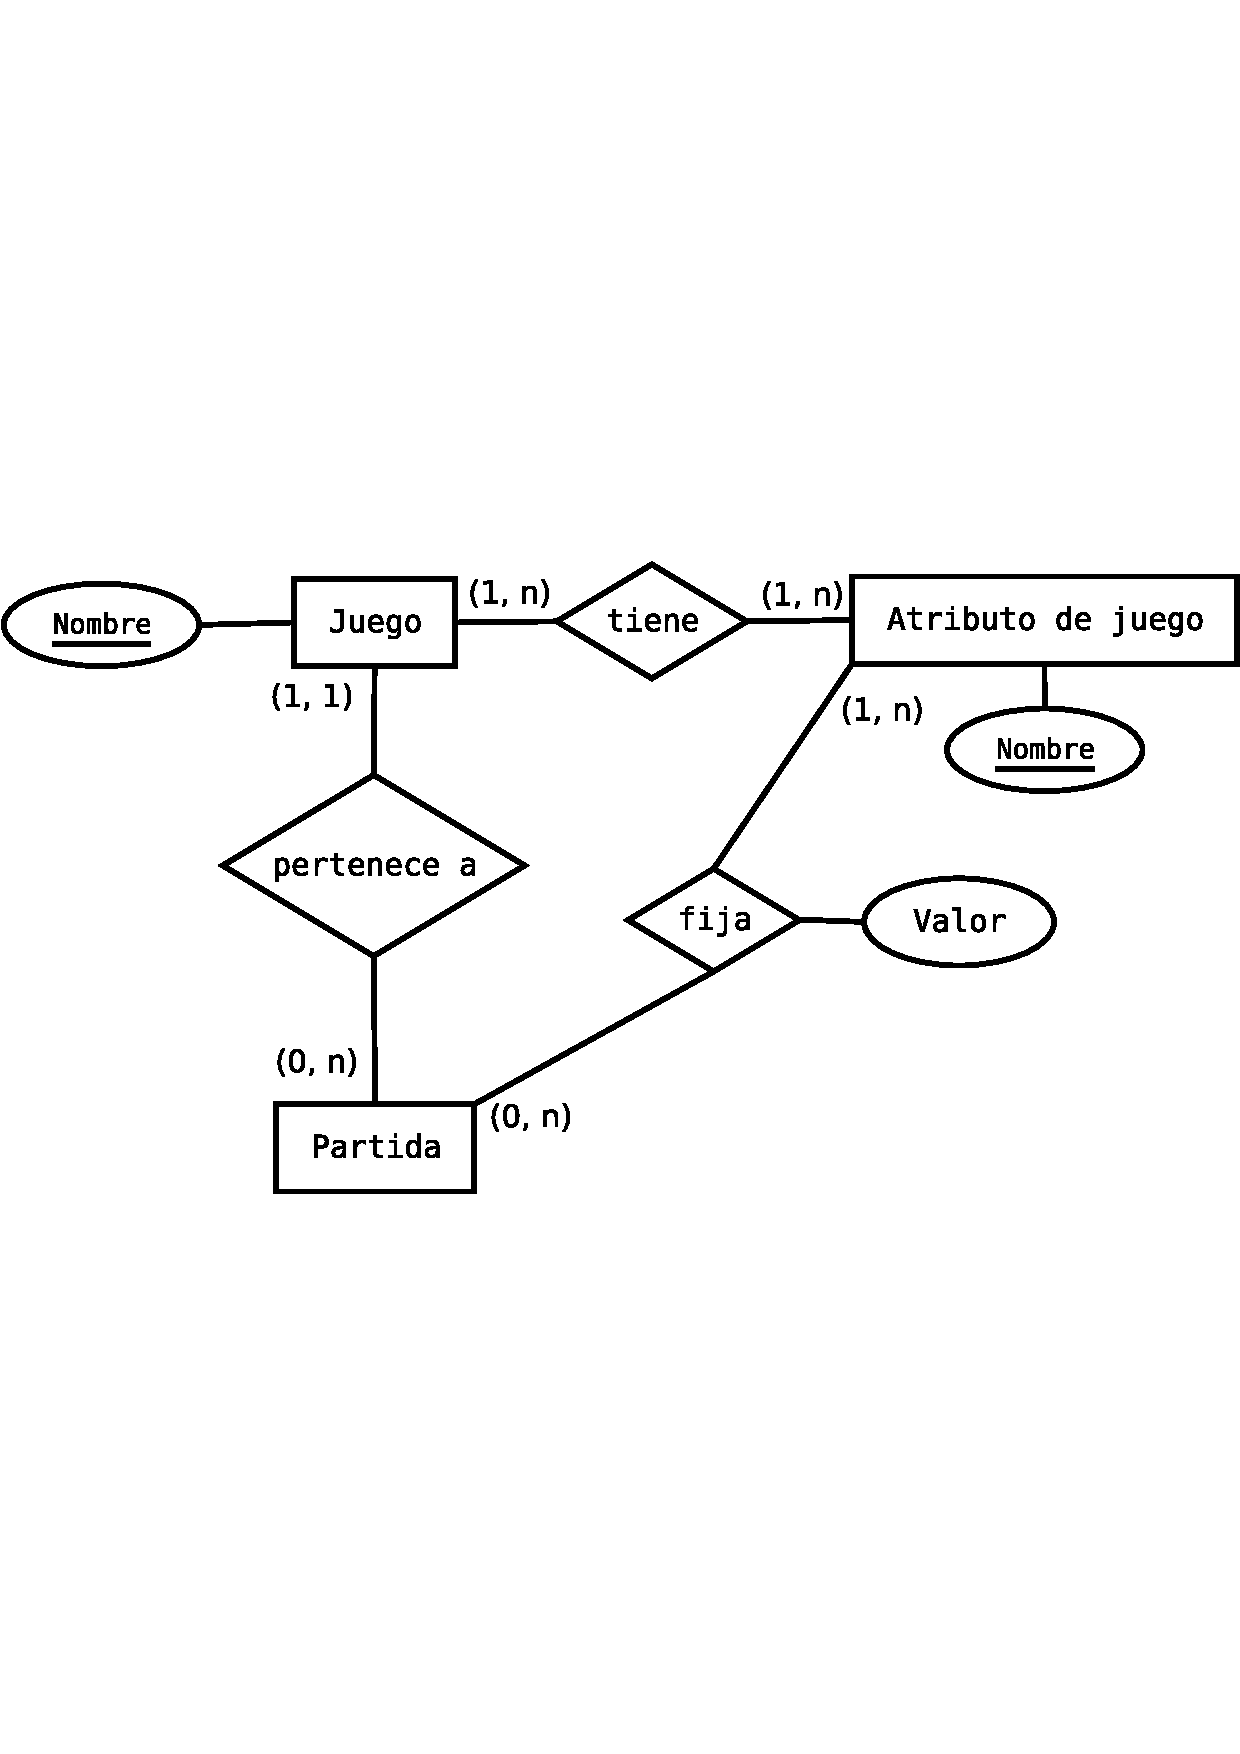
\includegraphics[width=0.7\linewidth]{../Diagramas/pdf/ER-Consulta.pdf}
	\caption{Diagrama ER del subsistema Consulta.}
	
	\label{fig:ERConsulta}
\end{figure}

\subsubsection{Diagramas de flujo de datos:}

Refinamos el proceso Consulta en sus cuatro requisitos funcionales  y realizando la descomposición del almacén en Partidas y Atributos mediante una primitiva descendente de descomposición en procesos sin conexiones.
 
\begin{figure}[h!]
\centering
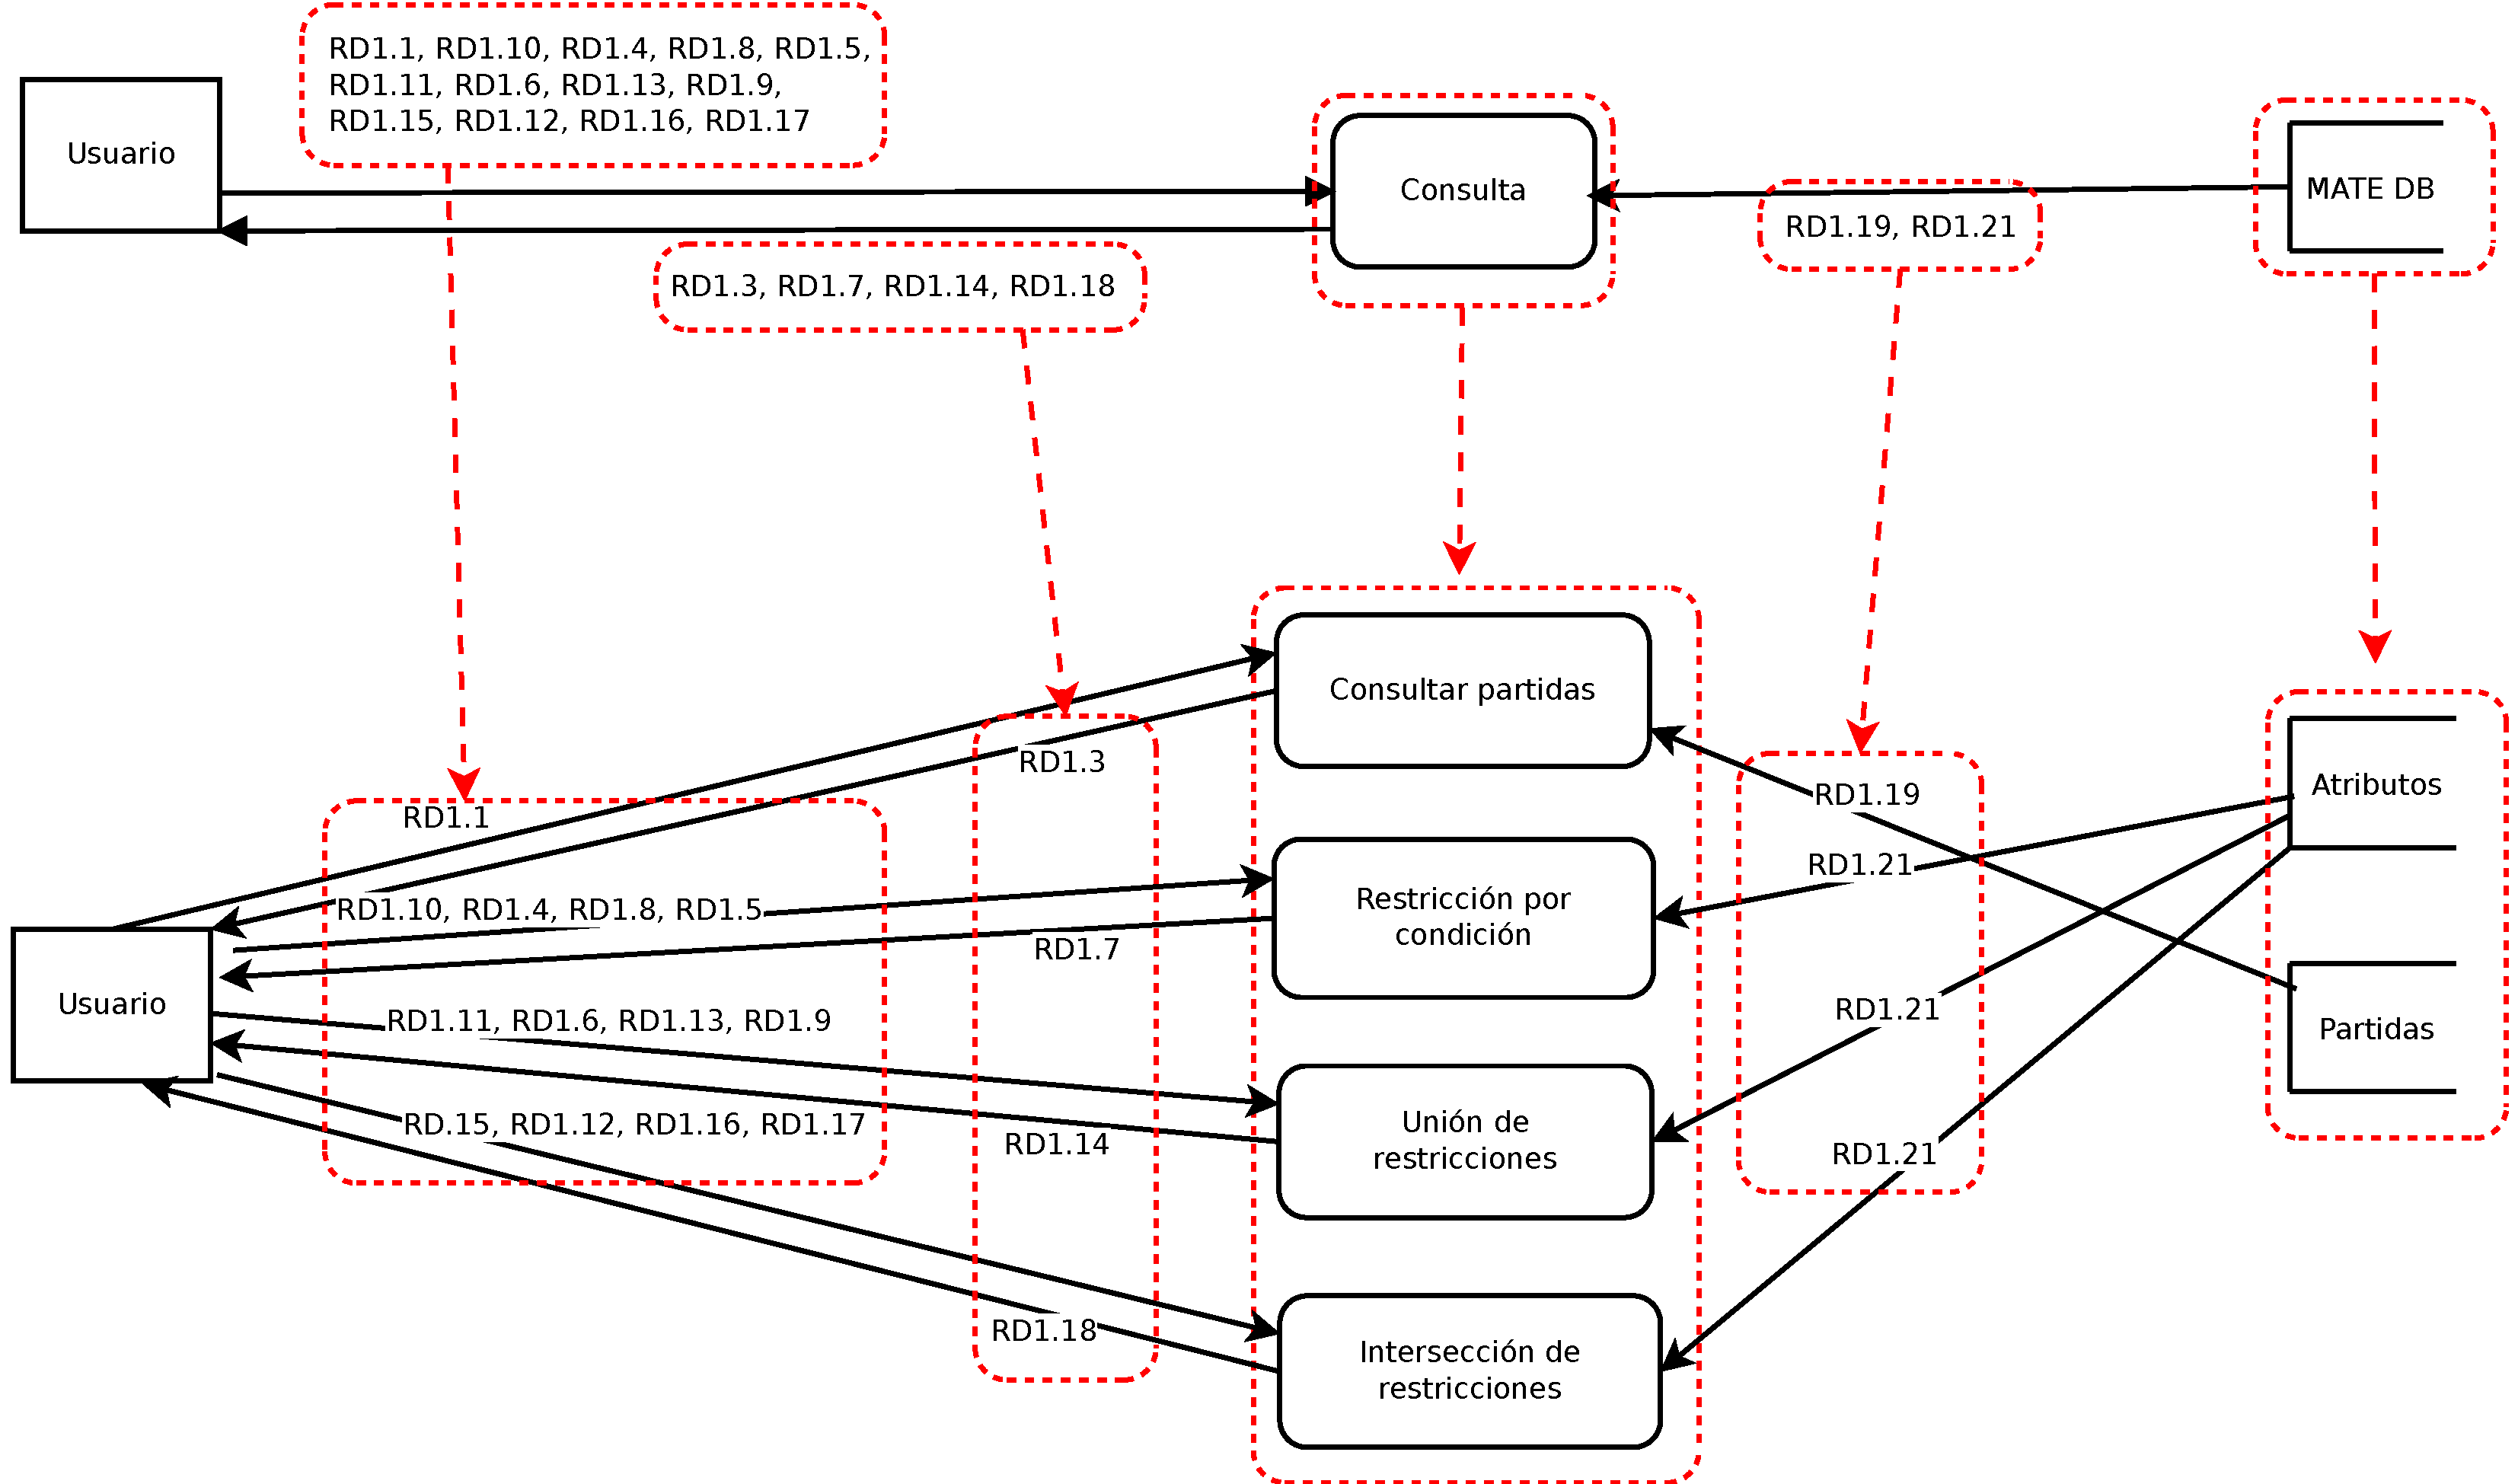
\includegraphics[width=0.7\linewidth]{../Diagramas/pdf/RefinamientoConsulta.pdf}
\caption{Flujo de datos del subsistema Consulta.}

\label{fig:RefinamientoConsulta}
\end{figure}

\subsubsection{Esquema Externo:}

\begin{figure}[h!]
	\centering
	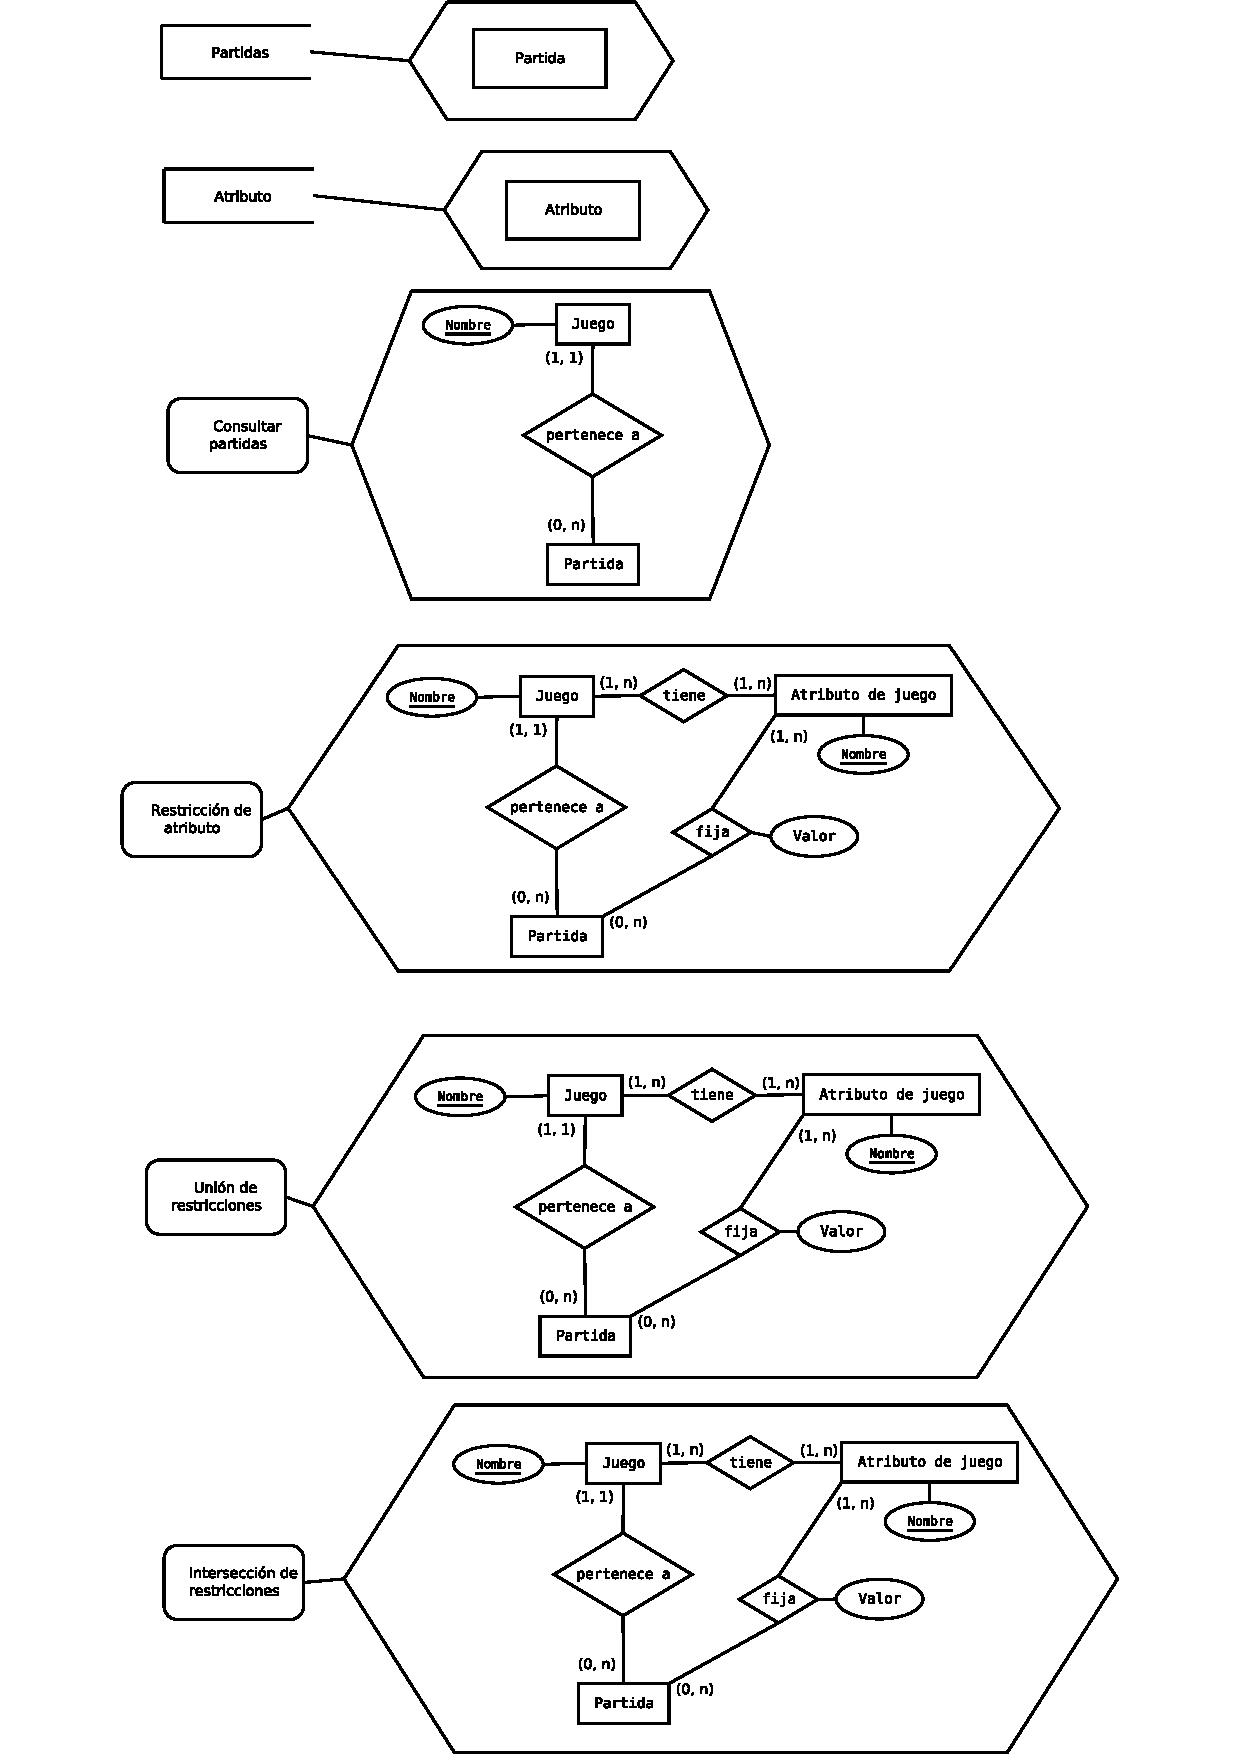
\includegraphics[width=0.7\linewidth]{../Diagramas/pdf/EsquemaExternoConsulta.pdf}
	\caption{Esquema externo de Consulta.}
	
	\label{fig:EsquemaExtConsulta}
\end{figure}


\subsection{Consejos (Bruno Santidrián)}
En todos los juegos en los que se guarde el estilo de juego, la aplicación
aconseja cómo jugar en determinadas condiciones, recomendando al usuario aquellos
estilos que más probabilidades tengan de ganar.\\

Dado un juego, el usuario podrá elegir uno o varios atributos de este (e.g. estilo
de juego en un partido de baloncesto: ofensivo o defensivo) y ciertos datos extra,
como el oponente al que se quiere enfrentar, o ciertos valores de los atributos 
que puede tener el oponente y el sistema analiza los datos guardados en la base
de datos para aconsejar unos valores que puedan ser beneficiosos (e.g. jugar ofensivo).\\

El subsistema debería dar información extra sobre el proceso de como ha elgido los
valores de los atributos, como el número de jugadas analizadas y la fiabilidad de los datos.\\

También es posible que el subsistema de consejos use funcionalidades del subsistema
de estadísticas, siempre que dicha funcionalidad esté implementada, para que las
recomendaciones sean más certeras.\\



\subsection{Inclusión de partidas (Darío Sierra)}
La inclusión de las partidas necesita que el usuario incluya aquellos atributos vitales en una partida, pudiendo o no incluir los opcionales. Necesitaría insertarlos por la interfaz gráfica.\\

El sistema de información que planteamos crear deberá incrementar el número de juegos disponibles con el avance del tiempo, para asegurar su uso continuado. Por tanto, distinguimos entre inclusión de juegos (trabajo de los administradores de la base de datos) y la inclusión de partidas (trabajo de los usuarios).\\

Una partida será un registro más de la tabla de datos asociada a cada juego. Como atributo vital se necesitará añadir el nombre del juego, así como la puntuación final de dicha partida; estos serán atributos comunes a cada a todas las partidas, pues todas pertenecerán a un juego y todas tendrán una puntuación asociada.\\

Los atributos opcionales serán aquellos inherentes a cada juego; no tiene sentido la inclusión de un atributo 'Jugadores del equipo' en un juego de cartas, ni un 'baraja del oponente' en uno que no lo sea. Aquí opcional no se entiende como 'poco relevante' pues estos atributos son la razón de ser del propio sistema de información. Los datos inherentes a cada juego, los que lo hacen distinguible del resto, serán objeto del análisis en el sistema.\\

Las partidas se incluirán desde la interfaz gráfica, donde una vez seleccionado el tipo de juego, se abrirán una serie de atributos (a definir por los administradores del sistema) que permitirán al jugador guardar su partida. Entre estos podremos encontrar: 'Jugadores del equipo', 'Mi Baraja', 'Baraja del oponente', 'Número de faltas cometido', 'Pichichi del encuentro', etc.\\

Aunque hemos clarificado que la inclusión de partidas debe ser trabajo de los usuarios, en juegos específicos (fútbol, baloncesto, etc), en los que, a diferencia de una partida entre dos jugadores de ajedrez, no queda claro quién debe almacenar el resultado. Es por esto, que se estudiará la posibilidad de responsabilizar a los administradores de mantener la base de datos actualizada para los juegos en los que se de esta situación.


\subsection{Estadísticas (Antonio Checa)}
Por último, el sistema debería agregar las estadísticas que pida el usuario. Hay diversos modos de generar una gráfica. El usuario tendrá que indicar al sistema qué modo de salida de los datos quiere (por ejemplo, una gráfica 2D con líneas). Una vez indicado, tendrá que añadir sobre qué atributos del juego quiere la gráfica de datos (por ejemplo, sobre la puntuación de los partidos de los Lakers en cada mes). Después, el sistema debe generar la representación elegida de los datos en caso de que pueda y presentarla ante el usuario. En caso de que no pueda deberá mostrar un mensaje de error mencionando la causa.

Los posibles modos de una gráfica son: gráfico 2D (al menos el eje Y debe ser numérico), gráfico 3D (al menos el eje Y debe ser numérico), columna agrupada (al menos dos elementos numéricos por cada uno no numérico), circular (atributos numéricos positivos).

Al tratar los atributos el usuario debe ser capaz de realizar funciones como la media, la suma o contar datos que cumplan una restricción concreta. Para esto, el sistema debe ser capaz de proporcionar ayuda con todas las funciones que se pueden insertar, y gestionarlas para que funcionen como es debido.


Las estadísticas, datos y gráficas generadas se tendrán que guardar en el sistema, para que el usuario pueda acceder a ellas sin tener que generarlas de nuevo. Habrá acceso a un registro con orden inverso a la fecha de creación para facilitar la búsqueda en el mismo.

Cada modo de salida tiene unas restricciones sobre los atributos, en el caso en el que el usuario incluya unos datos erróneos para una gráfica concreta (por ejemplo, seleccionar el modo de disco para representar datos que no son números). En este caso, el error tendrá que hacer referencia al error concreto, y mostrarlo por pantalla para que el usuario entienda qué ha pasado. 


\newpage
\section{Análisis de requisitos}

\subsection{Primer subsistema, consulta}
\subsubsection{Requisito de datos}

\begin{itemize}
	\item \textbf{RD1.1 Juego}. Se compone de:
	\begin{itemize}
		\item Un identificador de juego.
	\end{itemize}
	
	\item \textbf{RD1.2 Partida} de un juego.  Se compone de:
	\begin{itemize}
		\item Un identificador de partida.
	\end{itemize}
	
	\item \textbf{RD1.3 Partidas del juego}. Es en realidad todos los valores de todos los atributos de una partida, un valor por cada atributo. Cada valor puede ser de cualquier tipo, por ejemplo:
	\begin{itemize}
		\item Valor númerico.
		\item Una cadena de caracteres.
		\item Una letra.
		\item Una imagen.
		\item Un vídeo.
	\end{itemize}
	
	\item \textbf{RD1.4 Atributo} de una partida. Se encuentra añadido en la parte previa a la gestión de la base de datos.
	
	\item \textbf{RD1.5 Valor} de un atributo. Puede ser de cualquier tipo, por ejemplo:
	\begin{itemize}
		\item Valor númerico.
		\item Una cadena de caracteres.
		\item Una letra.
		\item Una imagen.
		\item Un vídeo.
	\end{itemize}
	
	\item \textbf{RD1.6 Atributos} de una partida. Es un conjunto de varios atributos añadidos en la parte previa a la gestión de la base de datos.
	
	\item \textbf{RD1.7 Valores de un mismo atributo}. Puede ser de cualquier tipo, aunque todos del mismo tipo, por ejemplo:
	\begin{itemize}
		\item Valor númerico.
		\item Una cadena de caracteres.
		\item Una letra.
		\item Una imagen.
		\item Un vídeo.
	\end{itemize}
	
	\item \textbf{RD1.8 Lista de condiciones}, de las cuales necesitan un valor de atributo, que son:
	\begin{itemize}
		\item 'sea menor que'.
		\item 'sea menor o igual que'.
		\item 'sea igual que'.
		\item 'sea mayor o igual que'.
		\item 'sea mayor que'.
		\item 'sea' (comparación entre cadena de caracteres).
		\item 'no sea' (comparación entre cadena de caracteres).
	\end{itemize}
	
	\item \textbf{RD1.9 Valores de varios atributos}. Pueden ser de cualquier tipo, por ejemplo:
	\begin{itemize}
		\item Valor númerico.
		\item Una cadena de caracteres.
		\item Una letra.
		\item Una imagen.
		\item Un vídeo.
	\end{itemize}
	
	\item \textbf{RD1.10 Juego}. Se compone de:
	\begin{itemize}
		\item Un identificador de juego.
	\end{itemize}
	
	\item \textbf{RD1.11 Juego}. Se compone de:
	\begin{itemize}
		\item Un identificador de juego.
	\end{itemize}
	
	\item \textbf{RD1.12 Atributos} de una partida. Es un conjunto de varios atributos añadidos en la parte previa a la gestión de la base de datos.
	
	\item \textbf{RD1.13 Lista de condiciones}, de las cuales necesitan un valor de atributo, que son:
	\begin{itemize}
		\item 'sea menor que'.
		\item 'sea menor o igual que'.
		\item 'sea igual que'.
		\item 'sea mayor o igual que'.
		\item 'sea mayor que'.
		\item 'sea' (comparación entre cadena de caracteres).
		\item 'no sea' (comparación entre cadena de caracteres).
	\end{itemize}
	
	\item \textbf{RD1.14 Valores de varios atributos}. Pueden ser de cualquier tipo, por ejemplo:
	\begin{itemize}
		\item Valor númerico.
		\item Una cadena de caracteres.
		\item Una letra.
		\item Una imagen.
		\item Un vídeo.
	\end{itemize}
	
	\item \textbf{RD1.15 Juego}. Se compone de:
	\begin{itemize}
		\item Un identificador de juego.
	\end{itemize}
	
	\item \textbf{RD1.16 Lista de condiciones}, de las cuales necesitan un valor de atributo, que son:
	\begin{itemize}
		\item 'sea menor que'.
		\item 'sea menor o igual que'.
		\item 'sea igual que'.
		\item 'sea mayor o igual que'.
		\item 'sea mayor que'.
		\item 'sea' (comparación entre cadena de caracteres).
		\item 'no sea' (comparación entre cadena de caracteres).
	\end{itemize}
	
	\item \textbf{RD1.17 Valores de varios atributos}. Pueden ser de cualquier tipo, por ejemplo:
	\begin{itemize}
		\item Valor númerico.
		\item Una cadena de caracteres.
		\item Una letra.
		\item Una imagen.
		\item Un vídeo.
	\end{itemize}
	
	\item \textbf{RD1.18 Valores de varios atributos}. Pueden ser de cualquier tipo, por ejemplo:
	\begin{itemize}
		\item Valor númerico.
		\item Una cadena de caracteres.
		\item Una letra.
		\item Una imagen.
		\item Un vídeo.
	\end{itemize}
	
	\item \textbf{RD1.19 Partidas} almacenadas de un juego concreto.
	
	\item \textbf{RD1.20 Partidas} almacenadas de un juego concreto.
	
	\item \textbf{RD1.21 Todos los valores de todos los atributos} almacenados de un juego concreto.
\end{itemize}




\subsubsection{Requisitos funcionales}
\begin{itemize}
	\item \textbf{RF1.1 Consultar partidas}: Consultar todas las partidas de un juego.
	
	Requisitos de entrada:
	\begin{itemize}
		\item RD1.1
	\end{itemize}
	Manejamiento de datos:
	\begin{itemize}
		\item RD1.19
	\end{itemize}
	Salida:
	\begin{itemize}
		\item RD1.3
	\end{itemize}
	
	
	\item \textbf{RF1.2 Restricción por condición}: Sobre un atributo, exigir que cumpla una condición dado un valor. Para facilitar esta función, sólo se puede exigir que se cumpla una condición sobre una lista de condiciones dada. Por ejemplo, Por ejemplo, si existiese un atributo en un juego que sólo tiene como valores {Ganado, Empatado, Perdido}, poder restringir a aquellas partidas donde dicho atributo sea 'Ganado'; o para el atributo 'Puntuación', poder elegir las partidas donde 'Se haya ganado por más de 10 puntos', donde la condición sobre el atributo 'Puntuación' sería 'es mayor que' y el valor pedido sería '10'.
	
	Requisitos de entrada: Se pasa el identificador del juego, el atributo a restringir, la lista de condiciones y el valor para la condición.
	\begin{itemize}
		\item RD1.10
		\item RD1.4
		\item RD1.8
		\item RD1.5
	\end{itemize}
	Manejamiento de datos: 
	\begin{itemize}
		\item RD1.21
	\end{itemize}
	Salida:
	\begin{itemize}
		\item RD1.7
	\end{itemize}
	
	
	\item \textbf{RF1.3 Unión de restricciones}: Poder hacer la función 'OR' entre restricciones en una consulta. Por ejemplo, 'todos los partidos en los que ganó o empató el Unicaja' o 'partidos en los que ganó el Unicaja o la diferencia en la puntuación fue menos de 10'.
	
	Requisitos de entrada: Se pasa el identificador del juego, los atributos a realizar la unión de restricciones, la lista de condiciones donde se selecciona una condición por atributo y los valores para cada condición.
	\begin{itemize}
		\item RD1.11
		\item RD1.6
		\item RD1.13
		\item RD1.9
	\end{itemize}
	Manejamiento de datos: 
	\begin{itemize}
		\item RD1.21
	\end{itemize}
	Salida:
	\begin{itemize}
		\item RD1.14
	\end{itemize}
	
	
	\item \textbf{RF1.4 Intersección de restricciones}: Poder hacer la función 'AND' entre restricciones en una consulta. Por ejemplo, 'todos los partidos en los que ganó y empató el Unicaja' o 'partidos en los que ganó el Unicaja y la diferencia en la puntuación fue menos de 10'.
	
	Requisitos de entrada: Se pasa el identificador del juego, los atributos a realizar la intersección de restricciones, la lista de condiciones donde se selecciona una condición por atributo y los valores para cada condición.
	\begin{itemize}
		\item RD1.15
		\item RD1.12
		\item RD1.16
		\item RD1.17
	\end{itemize}
	Manejamiento de datos: 
	\begin{itemize}
		\item RD1.21
	\end{itemize}
	Salida:
	\begin{itemize}
		\item RD1.18
	\end{itemize}
\end{itemize}




\subsubsection{Restricciones semánticas}

\textbf{RS1.1}. Para RF1.2, el valor de RD1.5 que acompaña a las concretas condiciones de 'es menor que', 'es menor o igual que', 'es igual que', 'es mayor o igual que', 'es mayor que' de la lista de condiciones RD1.8 ha de ser numérico.

\subsection{Segundo subsistema, consejos}
\subsubsection{Requisitos de datos}

	\begin{itemize}
		\item \textbf{RD2.1: Juego} sobre el que se va a aconsejar.
			Se require un identificador del juego.

		\item \textbf{RD2.2: Atributo} para el que se quiere consejo.
			Requiere un identificador del atributo.

		\item \textbf{RD2.3: Oponente} contra el que optimizar el atributo.
			Requiere un identificador del oponente.

		\item \textbf{RD2.4: Partidas del juego} almacenadas. 
			Se requerirán los campos que se considere que tienen información
			relevante para el consejo.

		\item \textbf{RD2.5: Valor del atributo} optimizado contra el oponente. 

		\item \textbf{RD2.6: Juego} sobre el que se va a aconsejar.
			Se require un identificador del juego.

		\item \textbf{RD2.7: Atributo} para el que se quiere consejo.
			Requiere un identificador del atributo.

		\item \textbf{RD2.8: Valor del atributo} optimizado contra todos los
			oponentes almacenados. 

		\item \textbf{RD2.9: Juego} sobre el que se va a aconsejar.
			Se require un identificador del juego.

		\item \textbf{RD2.10: Atributo} para el que se quiere consejo.
			Requiere un identificador del atributo.

		\item \textbf{RD2.11: Valor de los atributos} de un supuesto oponente.
			Consta de una lista de valores junto con el identificador del
			atributo al que esta asocido cada uno.

		\item \textbf{RD2.12: Valor del atributo} optimizado contra un oponente 
			con los atributos especificados. 
	\end{itemize}


\subsubsection{Requisitos funcionales}

	\begin{itemize}
		\item \textbf{RF2.1: Recomendar un atributo contra un oponente:} 
			El usuario selecciona un atributo del juego y un oponente y el
			sistema le proporciona un valor del atributo que probablemente
			sea beneficioso contra ese oponente.\\

			Requisitos de entrada:
			\begin{itemize}
				\item RD2.1 %juego
				\item RD2.2 %atributos
				\item RD2.3 %oponente
			\end{itemize}
			Manejo de datos:
			\begin{itemize}
				\item RD2.4 %partidas relevantes
			\end{itemize}
			Salida:
			\begin{itemize}
				\item RD2.5 %valor atributo
			\end{itemize}

		\item \textbf{RF2.2: Recomendar el mejor atributo en general:}
			El usuario selecciona un atributo del juego y el sistema le
			proporciona un valor del atributo que probablemente sea
			beneficioso en la mayoría de partidas que juegue.\\

			Requisitos de entrada:
			\begin{itemize}
				\item RD2.6 %juego
				\item RD2.7 %atributos
			\end{itemize}
			Manejo de datos:
			\begin{itemize}
				\item RD2.4 %partidas relevantes
			\end{itemize}
			Salida:
			\begin{itemize}
				\item RD2.8 %valor atributo
			\end{itemize}

		\item \textbf{RF2.3: Recomendar un atributo con contexto:}
			El usuario selecciona un atributo del juego y
			el valor de uno o varios atributos del adversrio y el sistema
			proporciona un valor para el atributo seleccionado que
			probablemente sean beneficioso contra un adversario con
			los atributos especificados.\\

			Requisitos de entrada:
			\begin{itemize}
				\item RD2.9 %juego
				\item RD2.10 %atributo
				\item RD2.11 %atributos oponente
			\end{itemize}
			Manejo de datos:
			\begin{itemize}
				\item RD2.4 %partidas relevantes
			\end{itemize}
			Salida:
			\begin{itemize}
				\item RD2.12 %valor atributo
			\end{itemize}

	\end{itemize}


\subsubsection{Restricciones semánticas}


\subsection{Tercer subsistema, inclusión}
%TODO
\subsubsection{Requisito de datos}

\begin{itemize}
	\item \textbf{RD3.1: Atributos Principales}, proporcionados por el usuario, se componen de:
	\begin{itemize}
		\item Puntuación de la partida.
		\item Nombre del juego
	\end{itemize}

	\item \textbf{RD3.2: Atributos Secundarios}, se componen de:
	\begin{itemize}
		\item Nombre
		\item Valor del atributo
	\end{itemize}
	La lista de atributos secundarios la definirań los administradores del sistema.

	\item \textbf{RD3.3 Identificador de partida} Asignado por el sistema.

	\item \textbf{RD3.4 Comentarios de otros jugadores} Se permitirá asociar un comentario a la partida de otro jugador.
	\begin{itemize}
	\item String con el comentario
	\item identificador de partida
	\end{itemize}

	\item \textbf{RD3.5 Registro de partida} Se compone de:
	\begin{itemize}
		\item Atributos principales (obligatorio)
		\item Atributos secundarios (opcionales)
		\item Identificador de partida (obligatorio)
		\item Comentario de otros jugadores (opcional)
	\end{itemize}

	\item \textbf{RD3.6 Modificador de un registro} compuesto de:
	\begin{itemize}
	\item Atributos secundarios
	\item identificador de partida
	\end{itemize}


\end{itemize}



\subsubsection{Requisitos funcionales}

\begin{itemize}

	\item \textbf{RF3.1 Inclusión de una partida}: El usuario inserta una pareja que consta de nombre de juego y puntuación, creando un nuevo registro de partida.

	Requisitos de entrada: Nombre del juego y puntuación
	\begin{itemize}
		\item RD3.1
	\end{itemize}

	Manejo de datos: Se leen los atributos, en caso de que el nombre del juego sea aceptado, se crea el registro.
	\begin{itemize}
		\item RD3.5
	\end{itemize}

	Salida: Identificador de la partida.
	\begin{itemize}
		\item RD3.3
	\end{itemize}

	\item \textbf{RF3.2 Modificación de un registro}: Una vez creado, el usuario podrá añadir atributos opcionales al registro.

	Requisitos de entrada: Lista de los atributos a insertar e identifificador de la partida.\\
	\begin{itemize}
		\item RD3.6
	\end{itemize}

	Manejo de datos: Se leen los atributos seleccionados y se insertan en el registro de la partida en cuestión. \\
	\begin{itemize}
		\item RD3.2
		\item RD3.5
	\end{itemize}

	Salida: A pantalla se muestra una interfaz en la que se representa el registro completo.
	\begin{itemize}
		\item RD3.5
	\end{itemize}

	\item \textbf{RF3.3 Eliminación de un registro} Se permitirá eliminar un resgitro en concreto si poseemos su identificador.

	Requisito de entrada: Identificador de la partida.
	\begin{itemize}
		\item RD3.3
	\end{itemize}

	Manejo de datos: Se busca el registro y se elimina de la base de datos. \\
	\begin{itemize}
		\item RD5.5
	\end{itemize}

	Salida: Mensaje de conformidad. \\

	\item \textbf{RF3.4 Comentar la partida de otro jugador}

	Requisito de entrada: String con el comentario.
	\begin{itemize}
		\item RD3.4
	\end{itemize}

	Manejo de datos: Se asocia un comentario a la partida de otro jugador
	\begin{itemize}
		\item RD3.5
	\end{itemize}

	Salida: Mensaje de conformidad \\

\end{itemize}

	\subsubsection{Restricciones semánticas}

	\begin{itemize}
		\item \textbf{RS3.1 La puntuación de una partida es una pareja (a,b) donde a y b son naturales.}
			\begin{itemize}
				\item RD3.1
				\item RF3.1
			\end{itemize}
		\item \textbf{RS3.2 El identificador de una partida será un entero.}
			\begin{itemize}
				\item RD3.3
				\item RF3.1
				\item RF3.3
			\end{itemize}

		\item \textbf{No se permitirá asociar un string vacío a la sección de comentarios de una partida.}
		\begin{itemize}
			\item RD3.4
			\item RF3.4
		\end{itemize}
	\end{itemize}


\subsection{Cuarto subsistema, estadísticas}
%TODO
\subsubsection{Requisito de datos}
\begin{itemize}
	\item \textbf{RD4.1: Atributos de entrada a una gráfica 2D}, proporcionados por el usuario, se componen de:
	\begin{itemize}
		\item Atributo de la partida sobre la X
		\item Atributo de la partida sobre la Y
	\end{itemize}
	
	\item \textbf{RD4.2: Atributos de una partida}, se componen de:
	\begin{itemize}
		\item Nombre
		\item Valor del atributo
	\end{itemize}
	
	\item \textbf{RD4.3: Gráfica 2D realizada}, se compone de:
	\begin{itemize}
		\item Imagen con la gráfica
	\end{itemize}
	
	\item \textbf{RD4.4: Atributos de entrada a una gráfica 3D}, se componen de:
	\begin{itemize}
			\item Atributo de la partida sobre la X
			\item Atributo de la partida sobre la Y
			\item Atributo de la partida sobre la Z
	\end{itemize}
	
	
	\item \textbf{RD4.5: Gráfica 3D}, se compone de:
	\begin{itemize}
			\item Imagen con la gráfica
	\end{itemize}
	
	\item \textbf{RD4.6: Atributos de entrada a una gráfica de columnas agrupadas}, se componen de:
	\begin{itemize}
		\item Atributo de la partida sobre la X
		\item Atributo de primer tipo de columna
		\item Atributo del segundo tipo de columna
	\end{itemize}
	
	\item \textbf{RD4.7: Gráfica de columnas agrupadas}, se compone de:
	\begin{itemize}
		\item Imagen con la gráfica
	\end{itemize}
	
	\item \textbf{RD4.8: Atributos de entrada a una gráfica circular}, se componen de:
	\begin{itemize}
		\item Atributo sobre el que se hace el círculo
	\end{itemize}
	
	\item \textbf{RD4.9: Gráfica circular}, se compone de:
	\begin{itemize}
			\item Imagen con la gráfica
	\end{itemize}
	
	\item \textbf{RD4.10: Atributo y función elemental}, se compone de:
	\begin{itemize}
		\item Atributo sobre el que se hace la función
		\item Función, a elegir, entre media, varianza, suma, contar, máximo o mínimo
	\end{itemize}
	
	\item \textbf{RD4.11: Resultado de la función}, se compone de:
	\begin{itemize}
		\item Resultado de la operación sobre el atributo
	\end{itemize}
	
	\item \textbf{RD4.12: Petición de conseguir las últimas gráficas}, se compone de:
	\begin{itemize}
		\item Activación de petición de la gráfica (pulsación de un botón)
	\end{itemize}
	
	\item \textbf{RD4.13: Gráficas anteriores}, se compone de:
	\begin{itemize}
		\item Imágenes de gráficas
	\end{itemize}
	
	\item \textbf{RD4.14: Gráficas anteriores como salida}, se compone de:
	\begin{itemize}
		\item Imágenes de gráficas
	\end{itemize}
	
	
	
	
	
\end{itemize}
\subsubsection{Requisitos funcionales}
\begin{itemize}
	\item \textbf{RF4.1 Realizar gráfica 2D de unos atributos}: El usuario selecciona dos atributos, de los cuales se realiza una gráfica 2D
	
	Requisitos de entrada: Elegir qué dos atributos se escogen
	\begin{itemize}
		\item RD4.1
	\end{itemize}
	Manejo de datos: Se leen los dos atributos seleccionados  y se inserta la gráfica en la base de datos
	\begin{itemize}
		\item RD4.2
	\end{itemize}
	Salida: Gráfica 2D
	\begin{itemize}
		\item RD4.3
	\end{itemize}
	
	\item \textbf{RF4.2 Realizar gráfica 3D de unos atributos}: El usuario selecciona tres atributos, de los cuales se realiza una gráfica 3D
	
	Requisitos de entrada: Elegir qué tres atributos se escogen
	\begin{itemize}
		\item RD4.4
	\end{itemize}
	Manejo de datos: Se leen los tres atributos seleccionados  y se inserta la gráfica en la base de datos
	\begin{itemize}
		\item RD4.2
	\end{itemize}
	Salida: Gráfica 3D
	\begin{itemize}
		\item RD4.5
	\end{itemize}
	
	\item \textbf{RF4.3 Realizar gráfica de columnas agrupadas de unos atributos}: El usuario selecciona dos atributos para las columnas y un tercero para el eje de abscisas, de los cuales se realiza la gráfica
	
	Requisitos de entrada: Elegir qué atributos se escogen
	\begin{itemize}
		\item RD4.6
	\end{itemize}
	Manejo de datos: Se leen los atributos seleccionados y se inserta la gráfica en la base de datos.
	\begin{itemize}
		\item RD4.2
	\end{itemize}
	Salida: Gráfica
	\begin{itemize}
		\item RD4.7
	\end{itemize}
	
	\item \textbf{RF4.4 Realizar gráfica circular de unos atributos}: El usuario selecciona un atributo, del cual se hace una gráfica porcentual en forma de círculo
	
	Requisitos de entrada: Elegir qué atributos se escoge.
	\begin{itemize}
		\item RD4.8
	\end{itemize}
	Manejo de datos: Se lee el atributo seleccionado y se inserta la gráfica en la base de datos.
	\begin{itemize}
		\item RD4.2
	\end{itemize}
	Salida: Gráfica.
	\begin{itemize}
		\item RD4.9
	\end{itemize}
	
	\item \textbf{RF4.5 Realizar una función elemental sobre un atributo concreto}: El usuario selecciona una función elemental (detalladas en la entrada de este requisito) y un atributo sobre el que operar, y se devuelve el resultado de la operación.
	
	Requisitos de entrada: El atributo y la función, a elegir entre media, varianza, suma, contar, máximo o mínimo.
	\begin{itemize}
		\item RD4.10
	\end{itemize}
	Manejo de datos: Se lee el atributo seleccionado y se opera.
	\begin{itemize}
		\item RD4.2
	\end{itemize}
	Salida: Resultado de la función.
	\begin{itemize}
		\item RD4.11
	\end{itemize}
	
	\item \textbf{RF4.6 Conseguir las últimas gráficas pedidas}: El usuario le da a un botón para ver las últimas gráficas que ha pedido.
	
	Requisitos de entrada: La activación de un botón.
	\begin{itemize}
		\item RD4.12
	\end{itemize}
	Manejo de datos: Se cogen las gráficas realizadas en función de su fecha.
	\begin{itemize}
		\item RD4.13
	\end{itemize}
	Salida: Gráficas, ordenadas de más a menos recientes.
	\begin{itemize}
		\item RD4.14
	\end{itemize}
	
\end{itemize}

\subsubsection{Restricciones semánticas}

\begin{itemize}
	\item \textbf{RS4.1 El atributo sobre la Y de RD4.1 sobre el requisito funcional de hacer una gráfica 2D RF4.1 debe ser de tipo numérico.}
	
	\item \textbf{RS4.2 El atributo sobre la Z de RD4.4 sobre el requisito funcional de hacer una gráfica 3D RF4.2 debe ser de tipo numérico.}
	
	\item \textbf{RS4.3 El atributo de los tipos de columnas en RD4.6 sobre el requisito funcional de hacer una gráfica de columnas agrupadas en RF4.3 deben ser de tipo numérico.}
	
	\item \textbf{RS4.4 El atributo de entrada a una gráfica circular en RD4.8 sobre el requisito funcional RF4.4 debe ser de tipo numérico y positivos.}
	
	\item \textbf{RS4.5 Los atributos de entrada a una función elemental en RD4.10 sobre el requisito funcional RF4.5 deben ser de tipo numérico.}
	
	
	
\end{itemize}

\newpage

\subsection{Diagramas conjuntos: Armazón y Caja Negra}
\begin{figure}
\centering
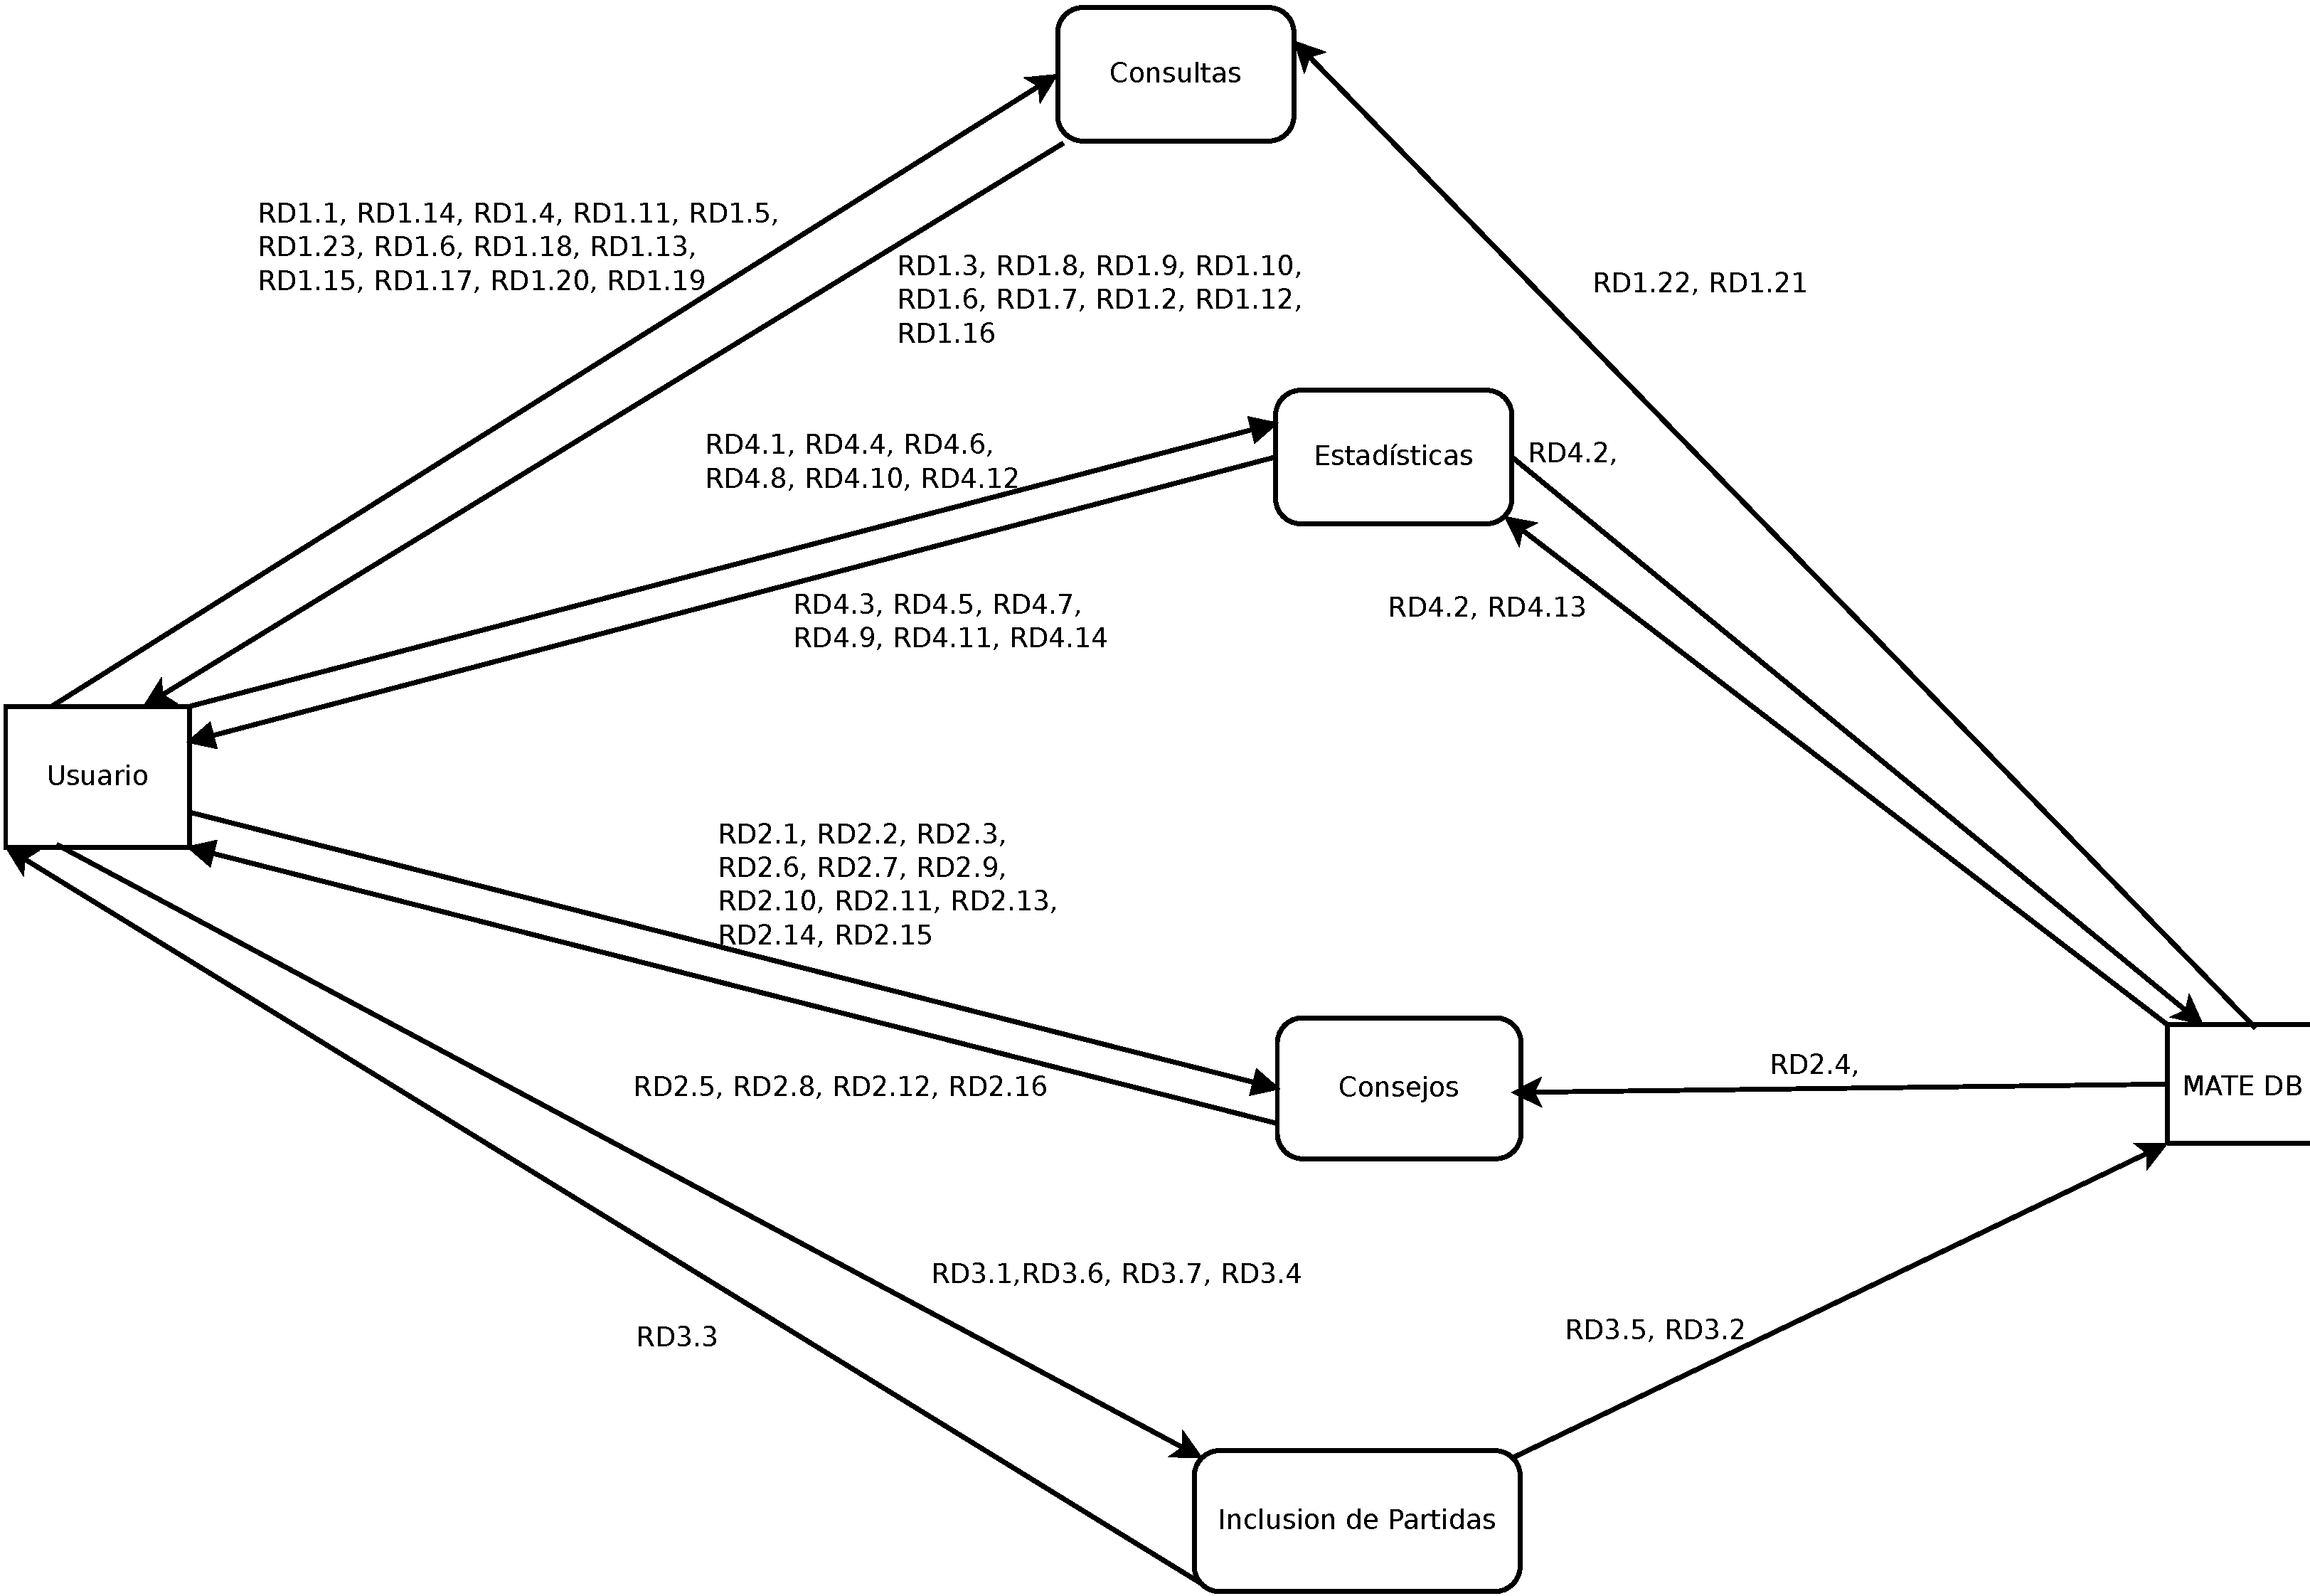
\includegraphics[width=0.7\linewidth]{../../Diagramas/pdf/Armazon.pdf}
\caption[Diagrama Armazón]{}
\caption{}
\label{fig:Armazon}
\end{figure}


\begin{figure}
\centering
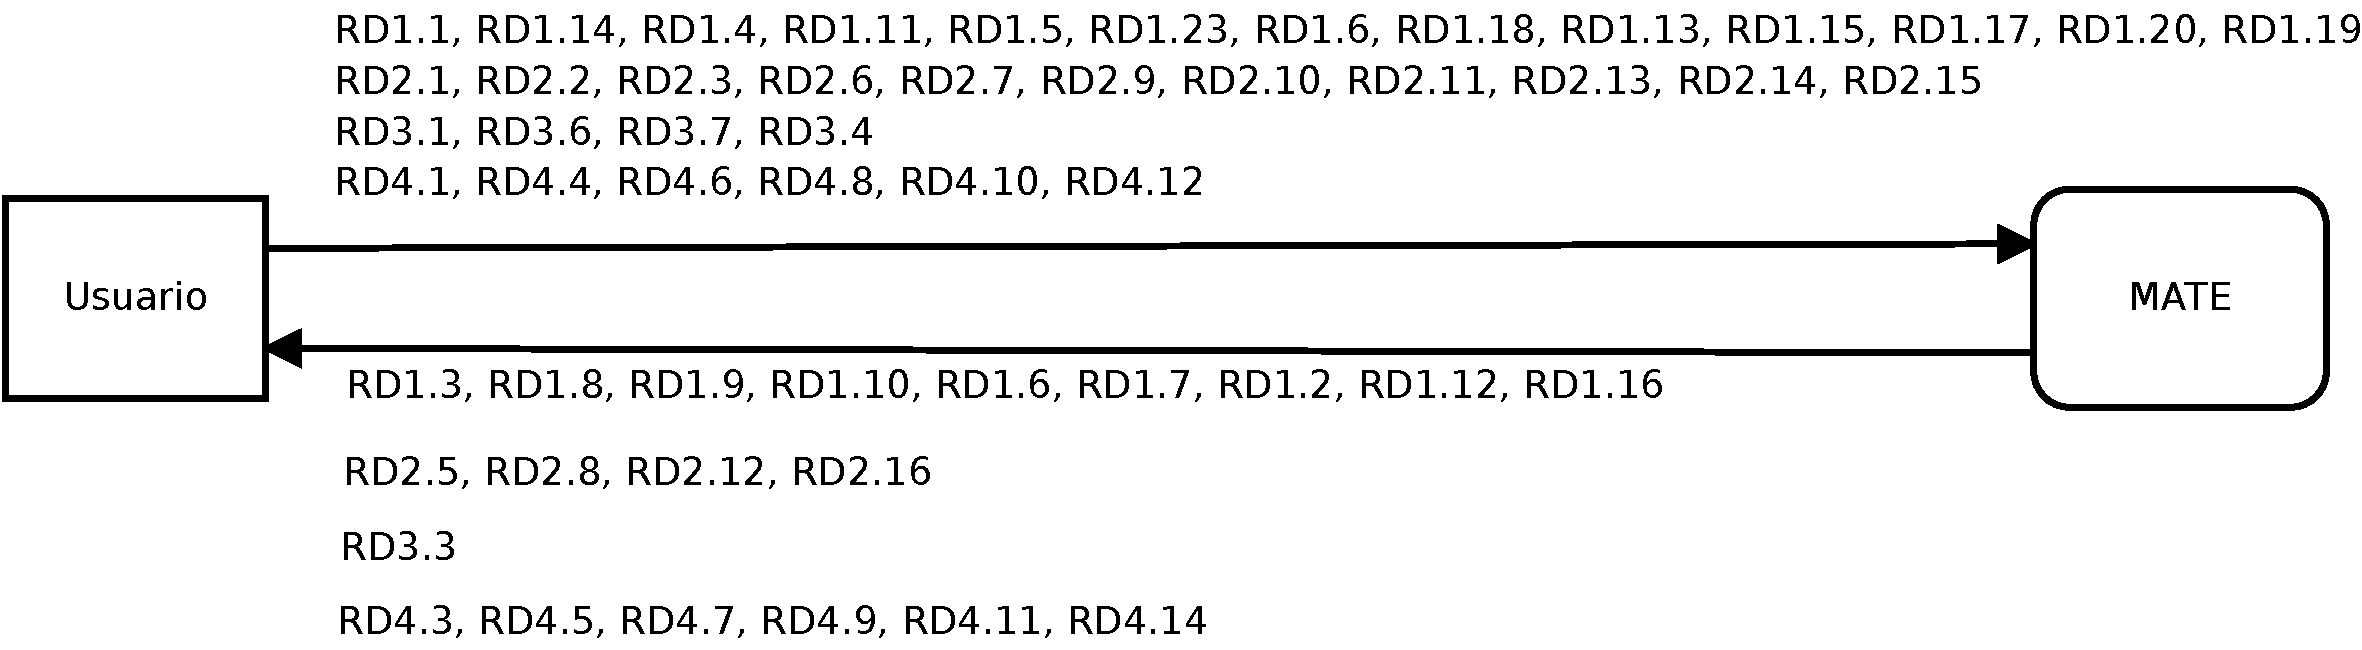
\includegraphics[width=0.7\linewidth]{../../Diagramas/pdf/CajaNegra.pdf}
\caption[Diagrama caja negra para el sistema MATE]{}
\caption{}
\label{fig:CajaNegra}
\end{figure}


\newpage
\subsection{Diagramas del primer subsistema, consulta}
\subsubsection{Esquema Entidad/Relación:}

\begin{figure}[h!]
	\centering
	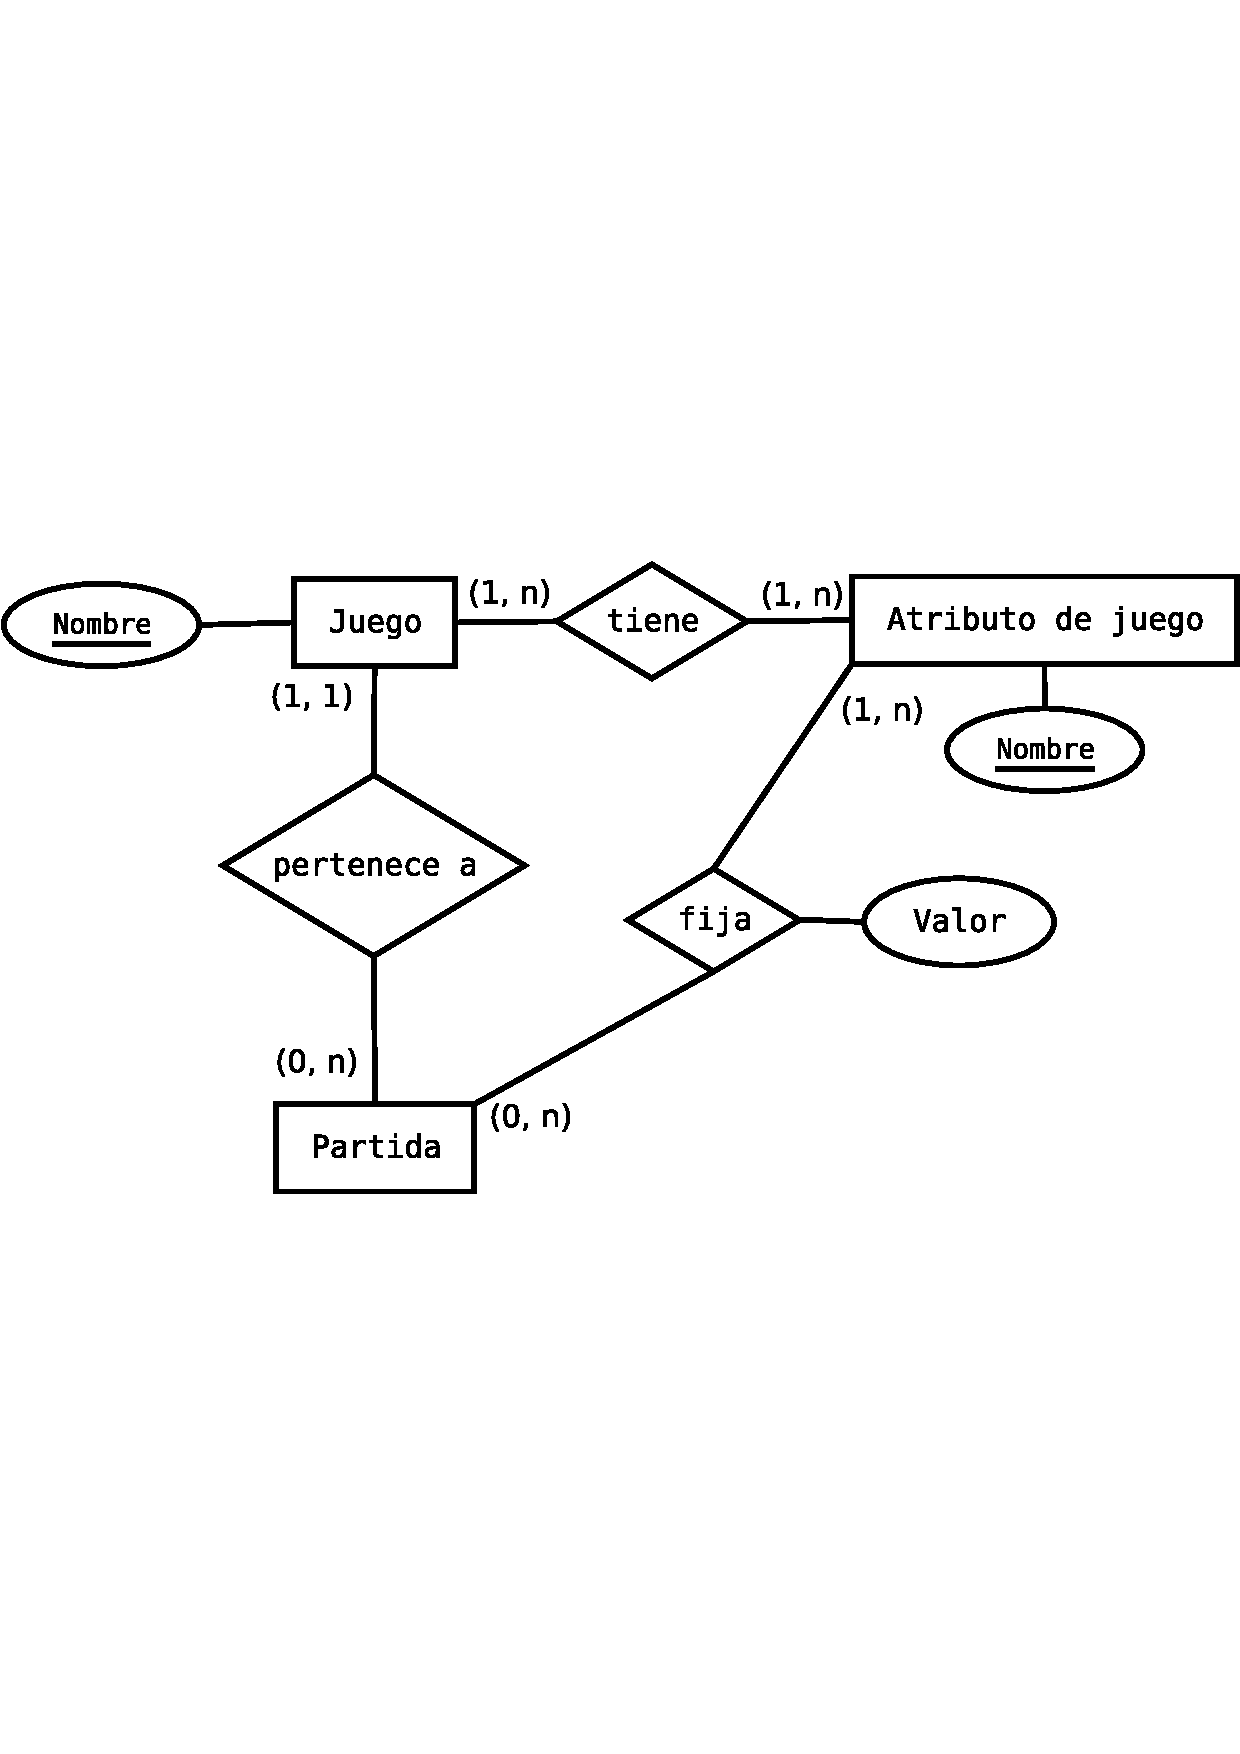
\includegraphics[width=0.7\linewidth]{../Diagramas/pdf/ER-Consulta.pdf}
	\caption{Diagrama ER del subsistema Consulta.}
	
	\label{fig:ERConsulta}
\end{figure}

\subsubsection{Diagramas de flujo de datos:}

Refinamos el proceso Consulta en sus cuatro requisitos funcionales  y realizando la descomposición del almacén en Partidas y Atributos mediante una primitiva descendente de descomposición en procesos sin conexiones.
 
\begin{figure}[h!]
\centering
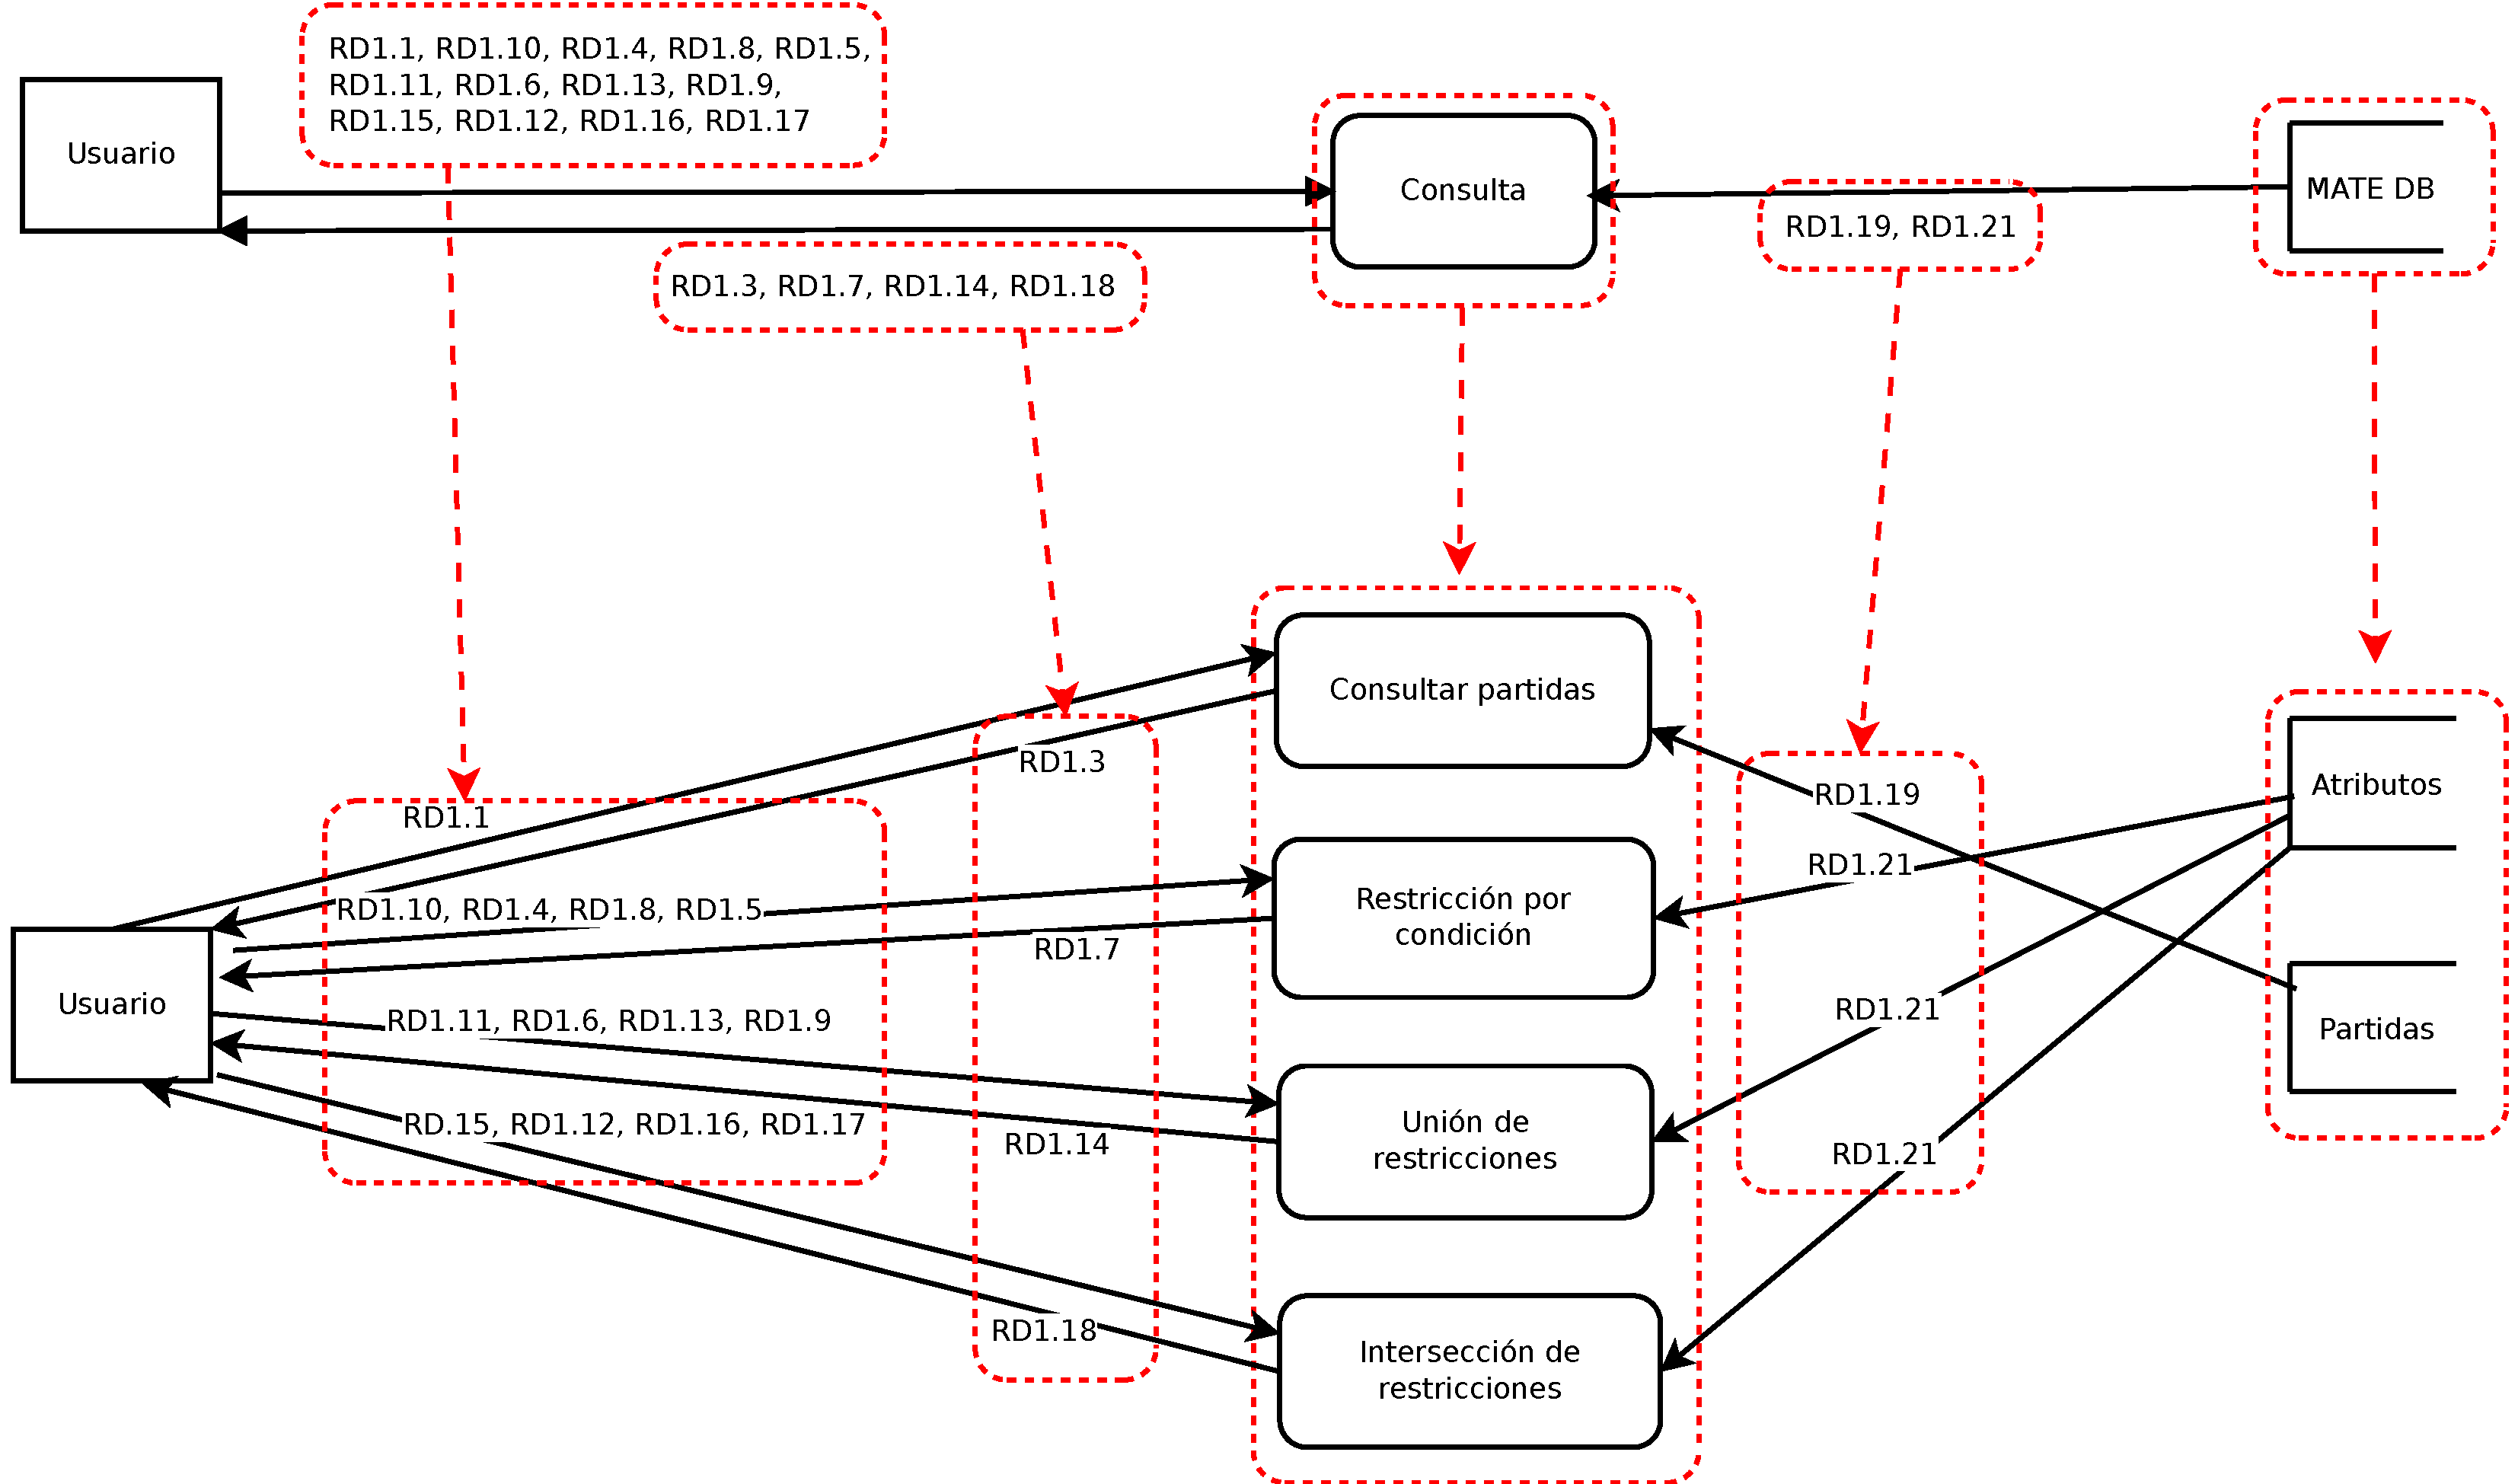
\includegraphics[width=0.7\linewidth]{../Diagramas/pdf/RefinamientoConsulta.pdf}
\caption{Flujo de datos del subsistema Consulta.}

\label{fig:RefinamientoConsulta}
\end{figure}

\subsubsection{Esquema Externo:}

\begin{figure}[h!]
	\centering
	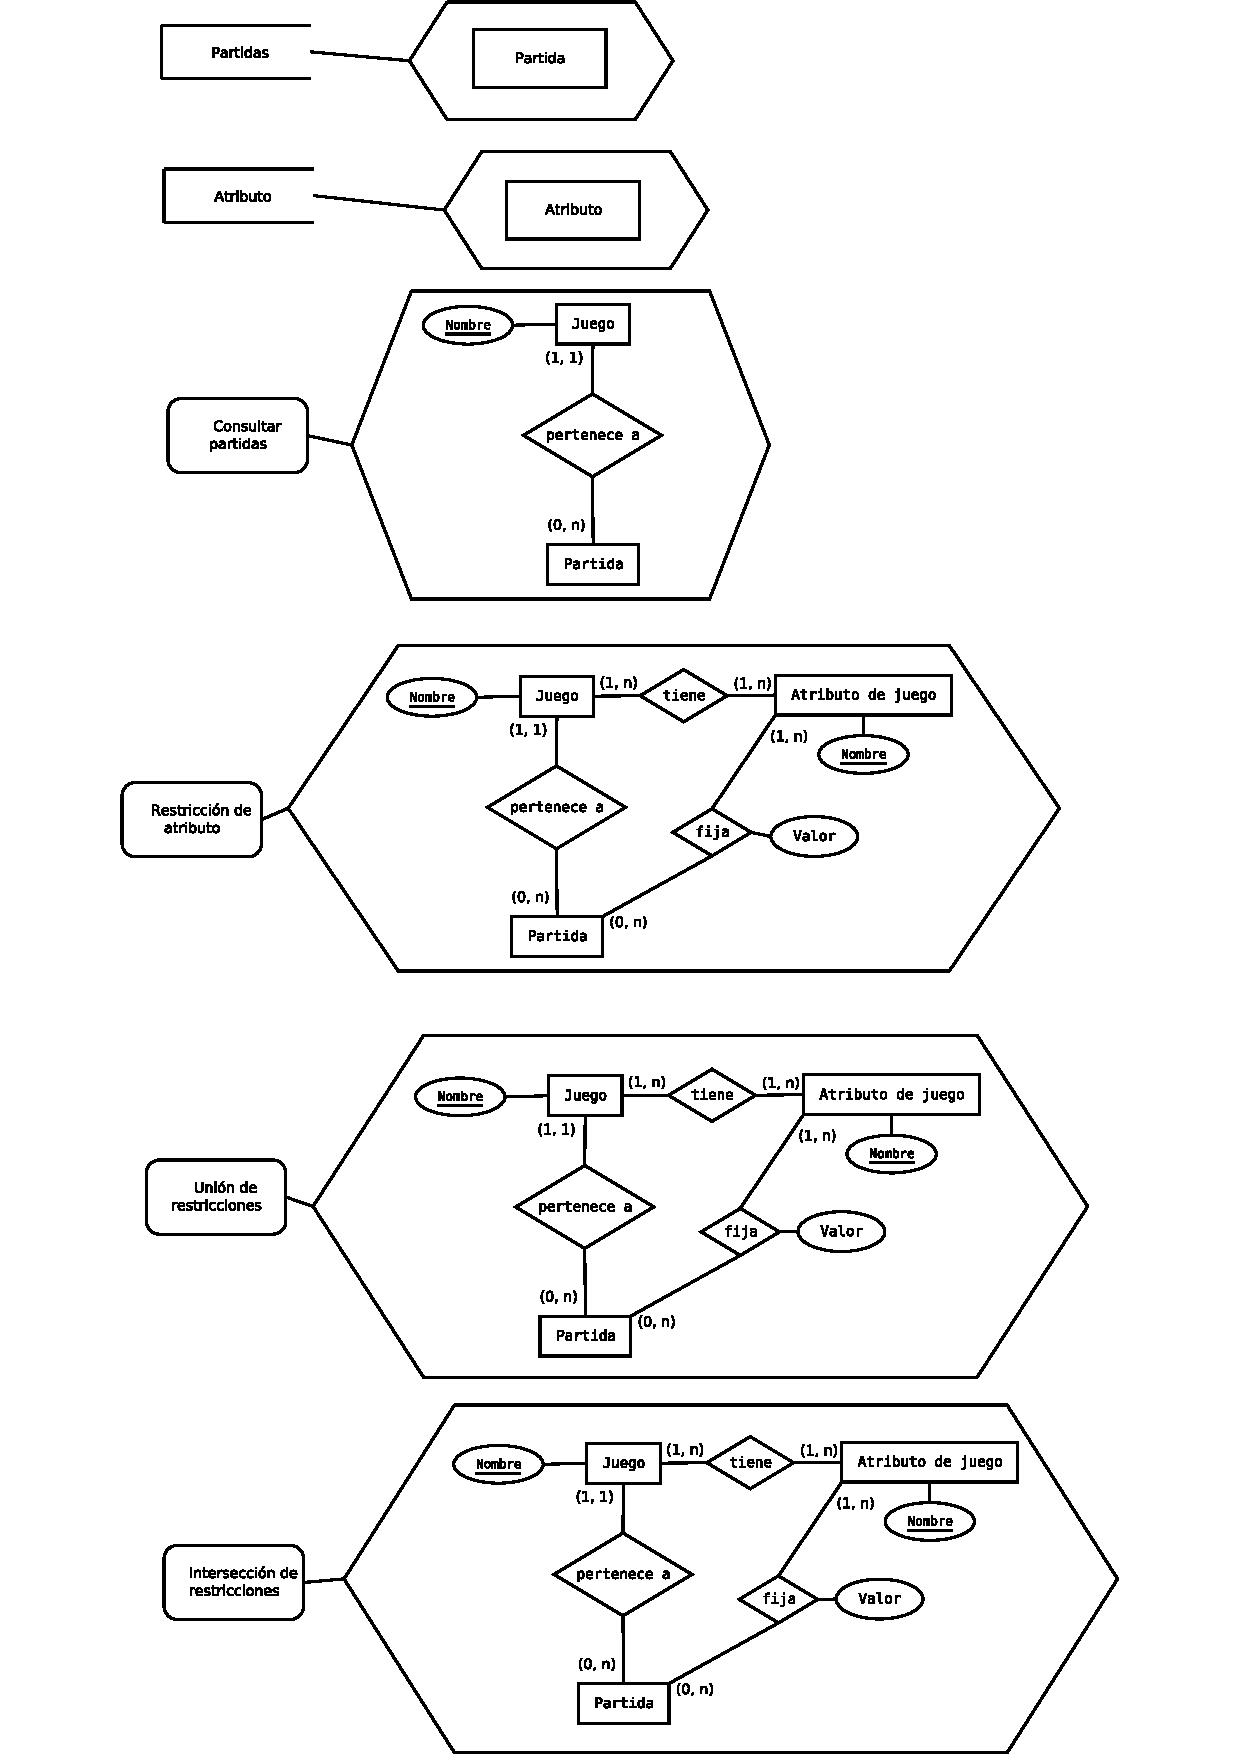
\includegraphics[width=0.7\linewidth]{../Diagramas/pdf/EsquemaExternoConsulta.pdf}
	\caption{Esquema externo de Consulta.}
	
	\label{fig:EsquemaExtConsulta}
\end{figure}


\newpage
\subsection{Diagramas del segundo subsistema, consejos}
En todos los juegos en los que se guarde el estilo de juego, la aplicación
aconseja cómo jugar en determinadas condiciones, recomendando al usuario aquellos
estilos que más probabilidades tengan de ganar.\\

Dado un juego, el usuario podrá elegir uno o varios atributos de este (e.g. estilo
de juego en un partido de baloncesto: ofensivo o defensivo) y ciertos datos extra,
como el oponente al que se quiere enfrentar, o ciertos valores de los atributos 
que puede tener el oponente y el sistema analiza los datos guardados en la base
de datos para aconsejar unos valores que puedan ser beneficiosos (e.g. jugar ofensivo).\\

El subsistema debería dar información extra sobre el proceso de como ha elgido los
valores de los atributos, como el número de jugadas analizadas y la fiabilidad de los datos.\\

También es posible que el subsistema de consejos use funcionalidades del subsistema
de estadísticas, siempre que dicha funcionalidad esté implementada, para que las
recomendaciones sean más certeras.\\



\newpage

\subsection{Diagramas del tercer subsistema, inclusión}

\begin{figure}[h!]
	\centering
	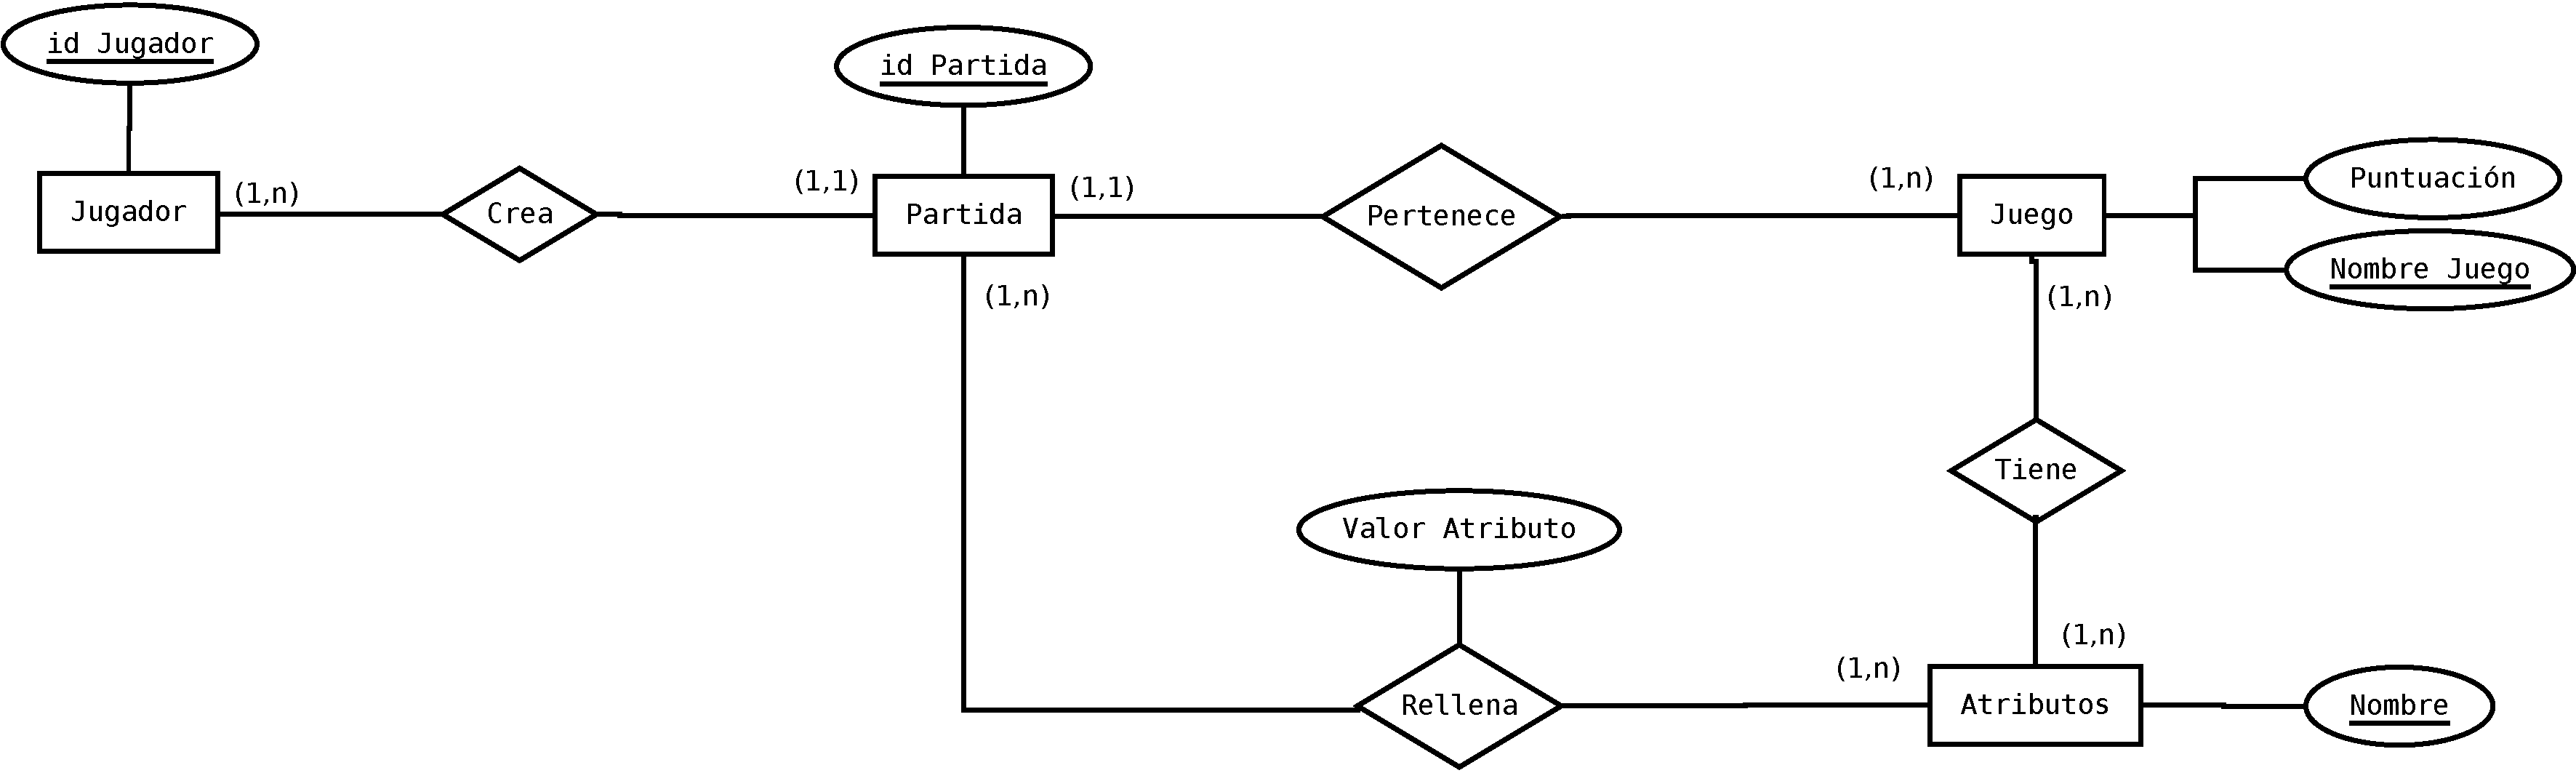
\includegraphics[width=0.7\linewidth]{../Diagramas/pdf/ER-Inclusion.pdf}
	\caption{Diagrama entidad relación del sistema de inclusión}
	\label{fig:ER}
\end{figure}



\begin{figure}[h!]
\centering
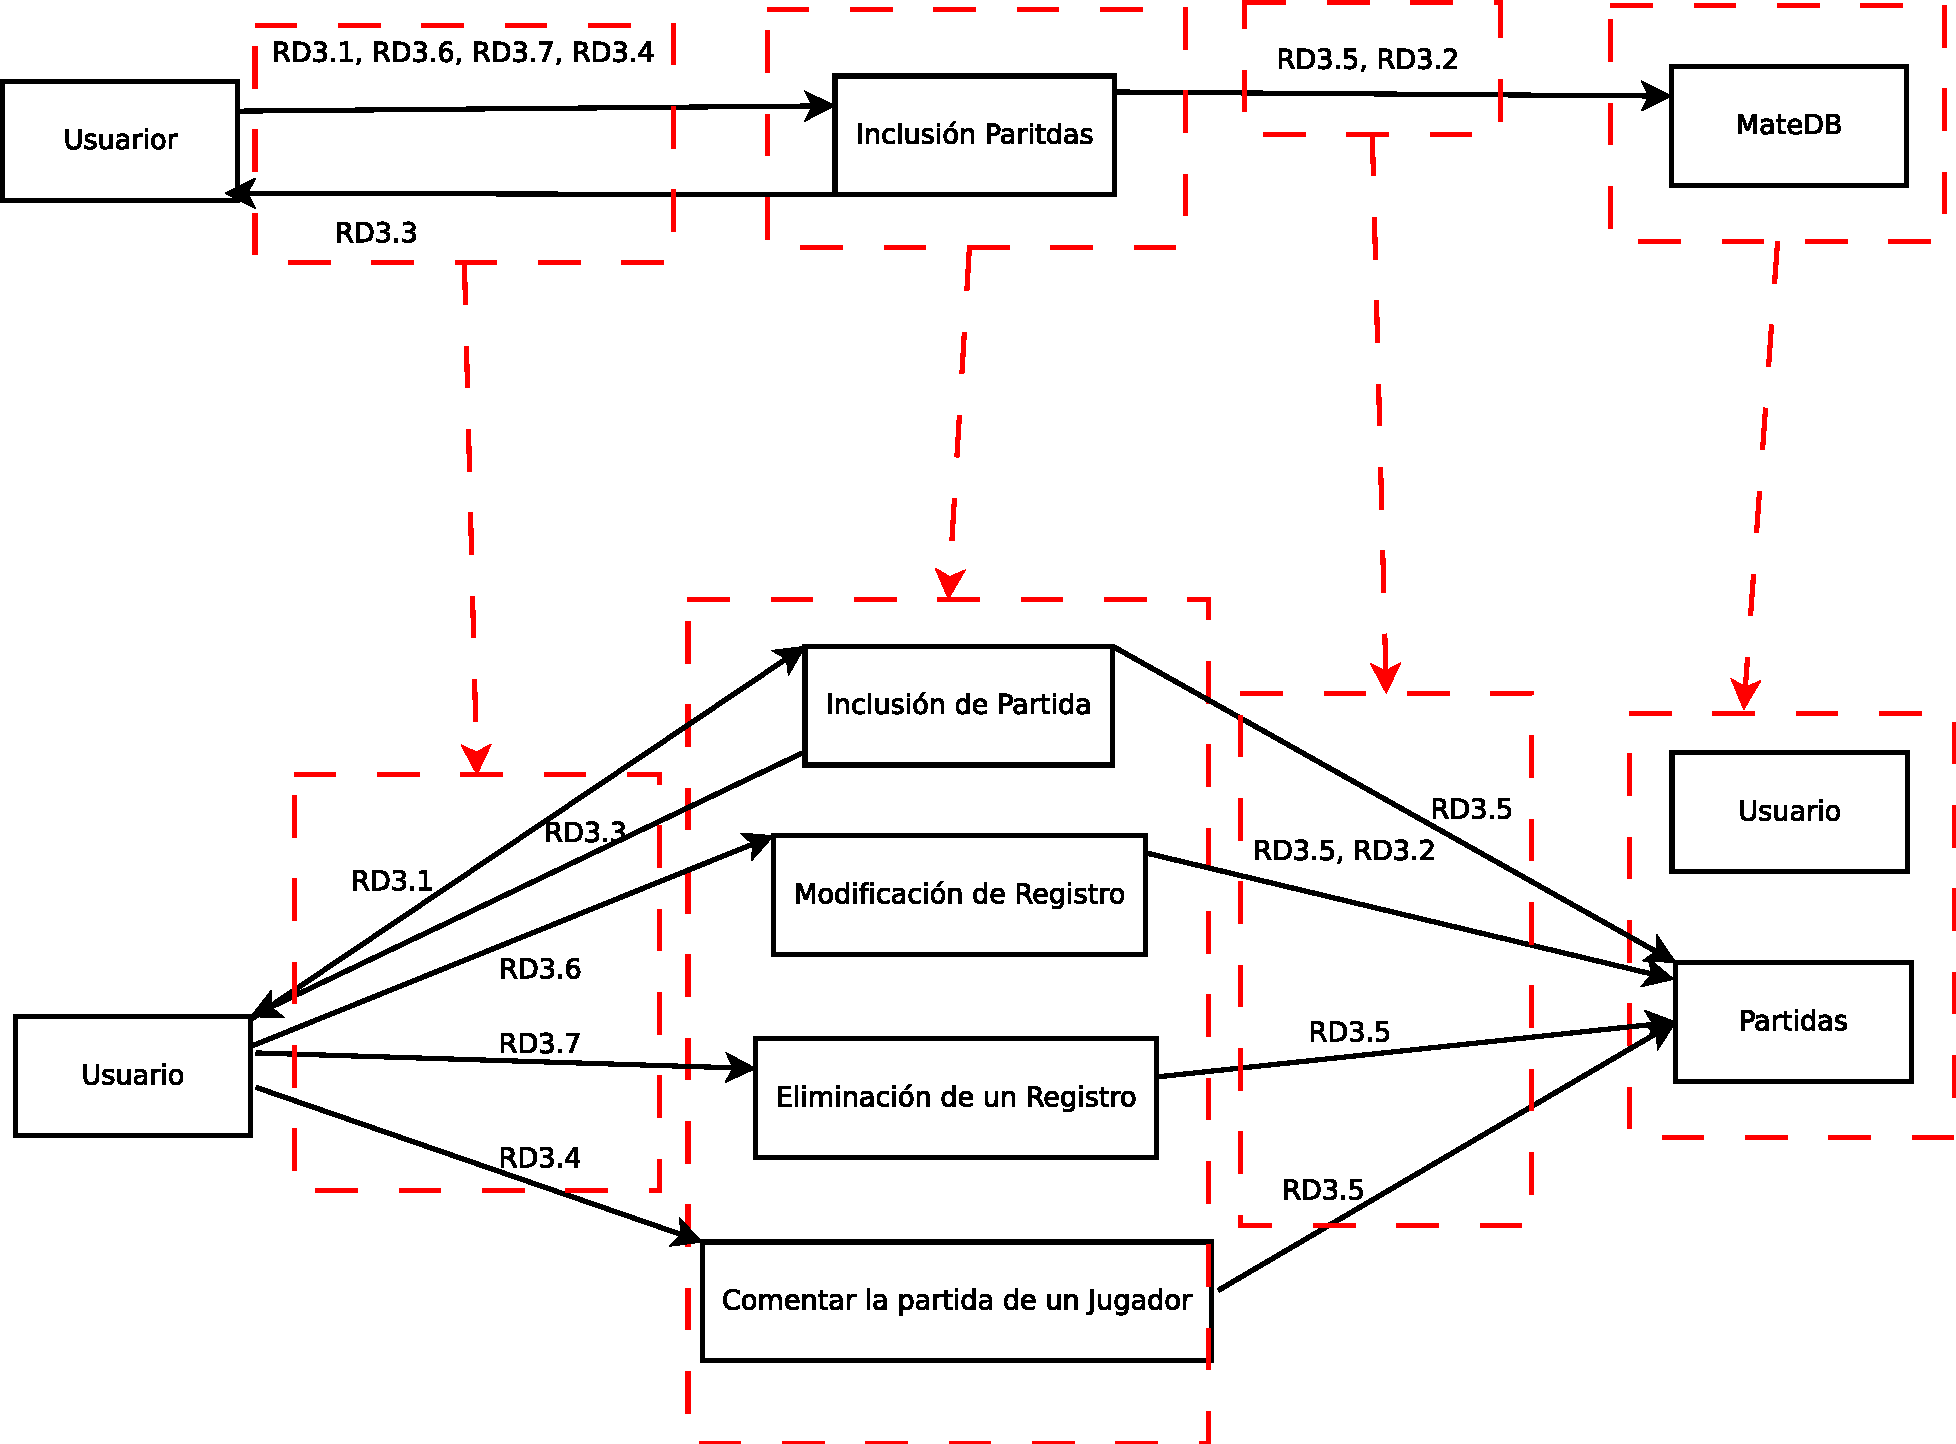
\includegraphics[width=0.7\linewidth]{../Diagramas/pdf/RefinamientoInclusion.pdf}
\caption{Refinamiento del sistema de inclusión}
\label{fig:RefinamientoInclusion}
\end{figure}


\subsection{Operaciones y almacenes del subsistema de inclusión}
\begin{figure}[H]
  \centering
  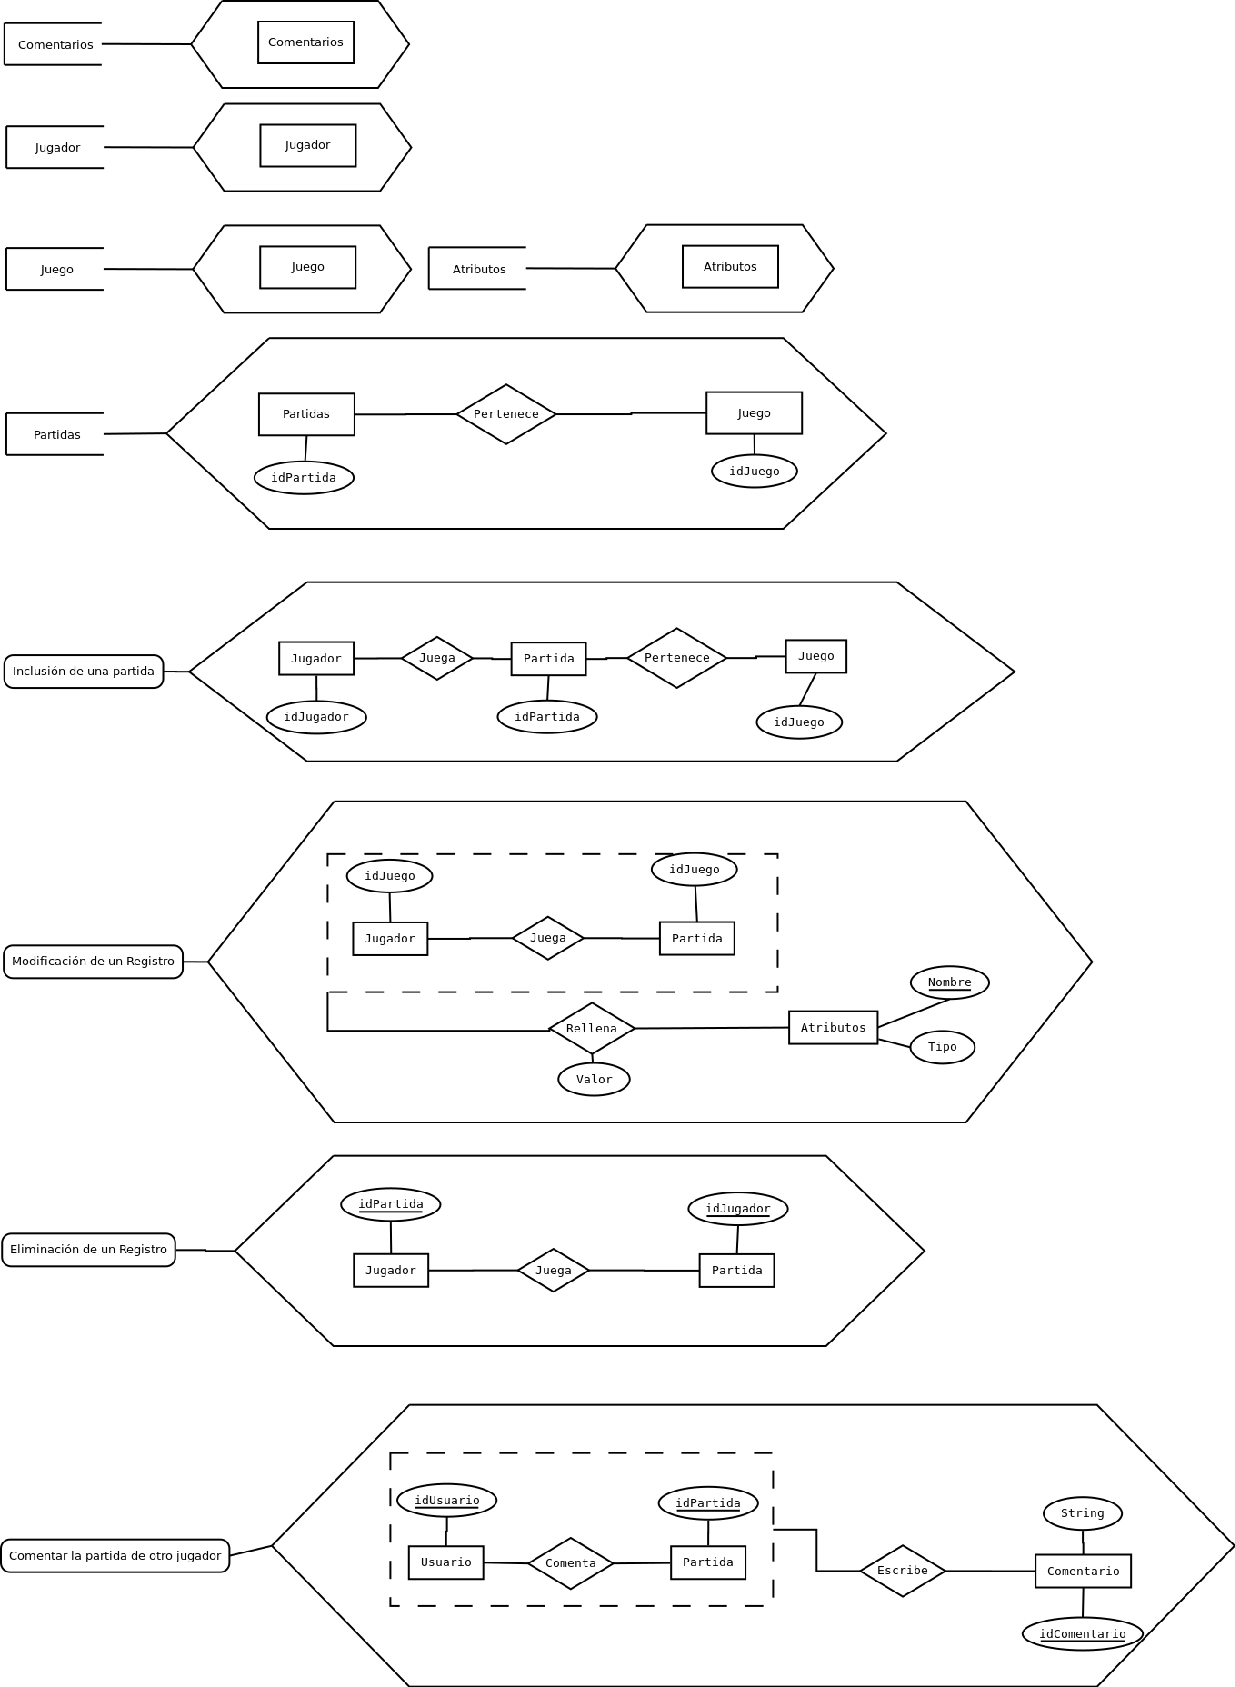
\includegraphics[width=0.5\linewidth]{../Diagramas/pdf/EsquemaExternoInclusion.pdf}
  \caption{Esquema de navegabilidad de O1 del proceso 1}
\end{figure}



\newpage


\subsection{Diagramas del cuarto subsistema, estadísticas}
Por último, el sistema debería agregar las estadísticas que pida el usuario. Hay diversos modos de generar una gráfica. El usuario tendrá que indicar al sistema qué modo de salida de los datos quiere (por ejemplo, una gráfica 2D con líneas). Una vez indicado, tendrá que añadir sobre qué atributos del juego quiere la gráfica de datos (por ejemplo, sobre la puntuación de los partidos de los Lakers en cada mes). Después, el sistema debe generar la representación elegida de los datos en caso de que pueda y presentarla ante el usuario. En caso de que no pueda deberá mostrar un mensaje de error mencionando la causa.

Los posibles modos de una gráfica son: gráfico 2D (al menos el eje Y debe ser numérico), gráfico 3D (al menos el eje Y debe ser numérico), columna agrupada (al menos dos elementos numéricos por cada uno no numérico), circular (atributos numéricos positivos).

Al tratar los atributos el usuario debe ser capaz de realizar funciones como la media, la suma o contar datos que cumplan una restricción concreta. Para esto, el sistema debe ser capaz de proporcionar ayuda con todas las funciones que se pueden insertar, y gestionarlas para que funcionen como es debido.


Las estadísticas, datos y gráficas generadas se tendrán que guardar en el sistema, para que el usuario pueda acceder a ellas sin tener que generarlas de nuevo. Habrá acceso a un registro con orden inverso a la fecha de creación para facilitar la búsqueda en el mismo.

Cada modo de salida tiene unas restricciones sobre los atributos, en el caso en el que el usuario incluya unos datos erróneos para una gráfica concreta (por ejemplo, seleccionar el modo de disco para representar datos que no son números). En este caso, el error tendrá que hacer referencia al error concreto, y mostrarlo por pantalla para que el usuario entienda qué ha pasado. 


\newpage
\section{Operaciones de datos}

\subsection{Primer subsistema, consulta}
\subsubsection{Esquema Entidad/Relación:}

\begin{figure}[h!]
	\centering
	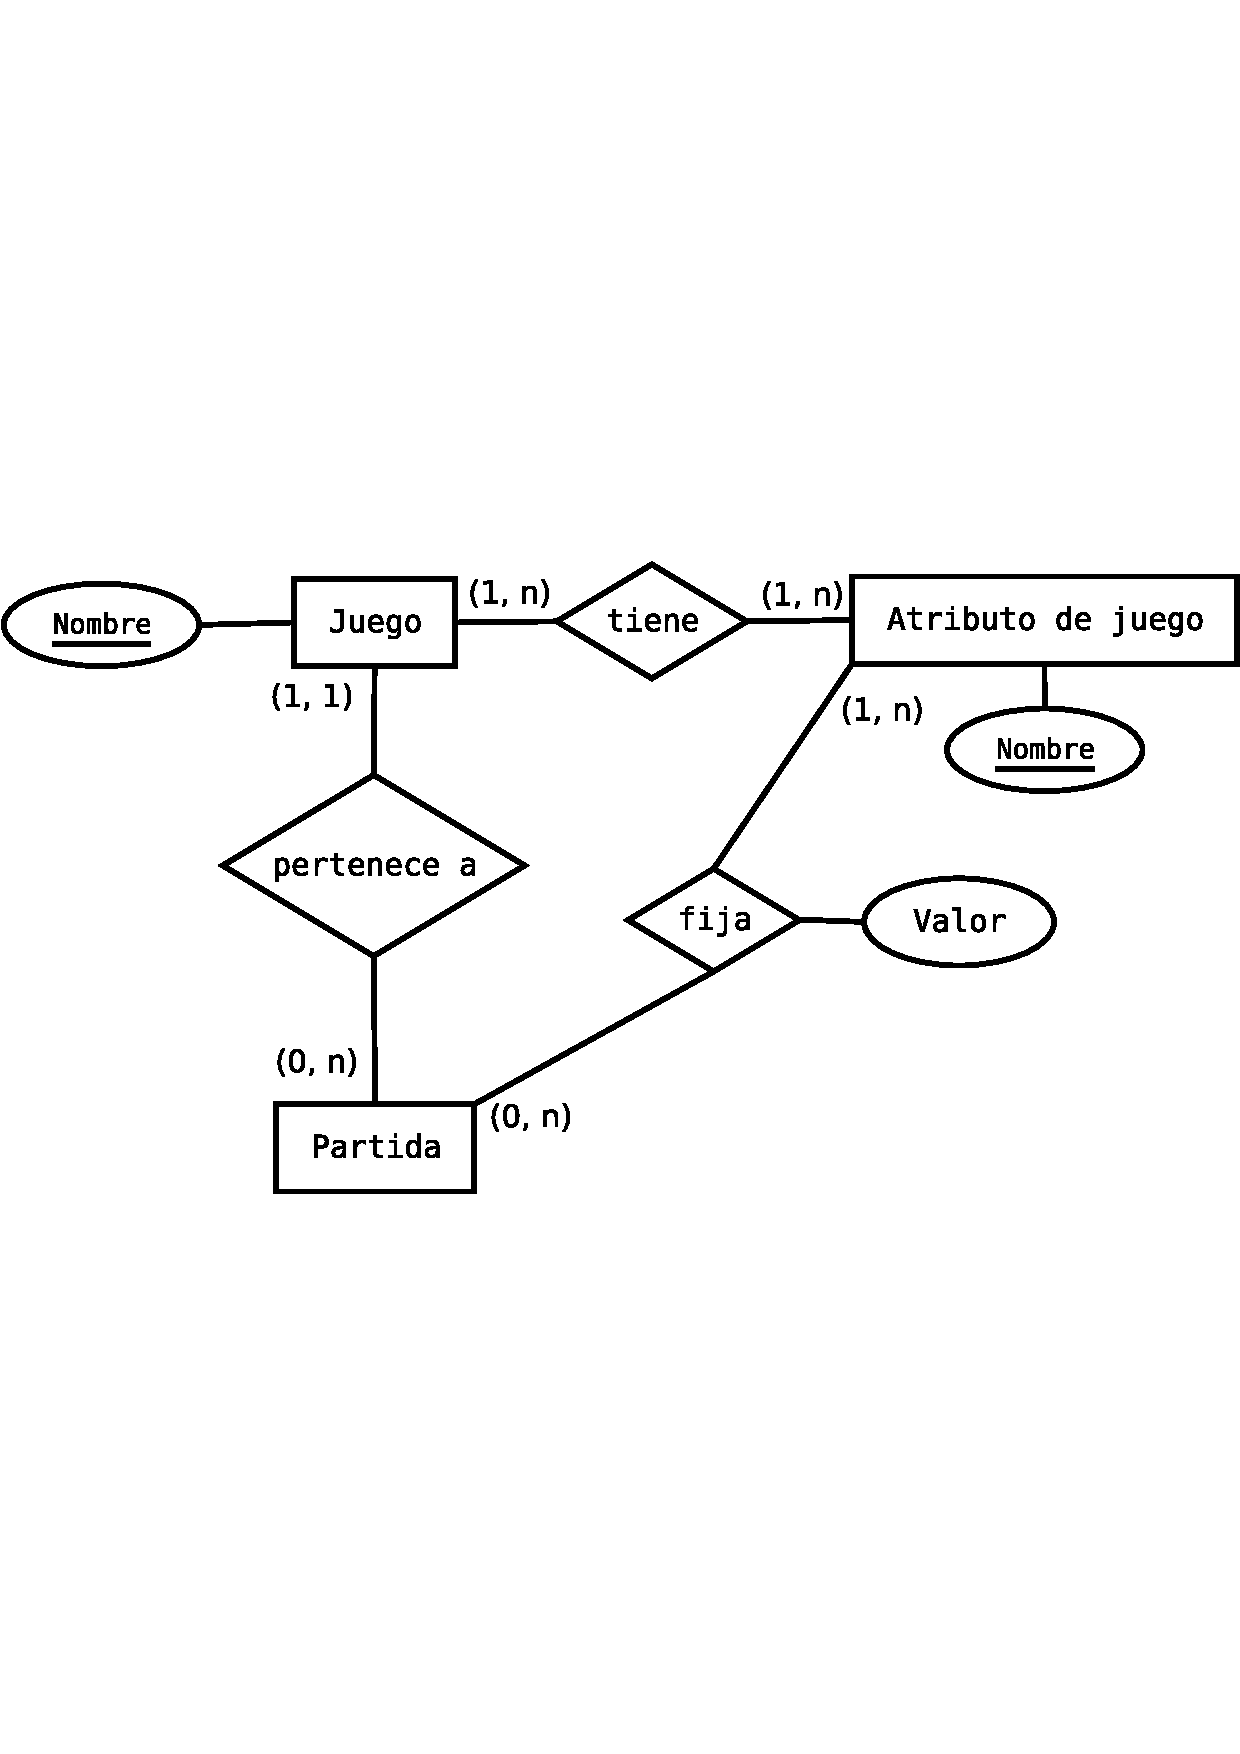
\includegraphics[width=0.7\linewidth]{../Diagramas/pdf/ER-Consulta.pdf}
	\caption{Diagrama ER del subsistema Consulta.}
	
	\label{fig:ERConsulta}
\end{figure}

\subsubsection{Diagramas de flujo de datos:}

Refinamos el proceso Consulta en sus cuatro requisitos funcionales  y realizando la descomposición del almacén en Partidas y Atributos mediante una primitiva descendente de descomposición en procesos sin conexiones.
 
\begin{figure}[h!]
\centering
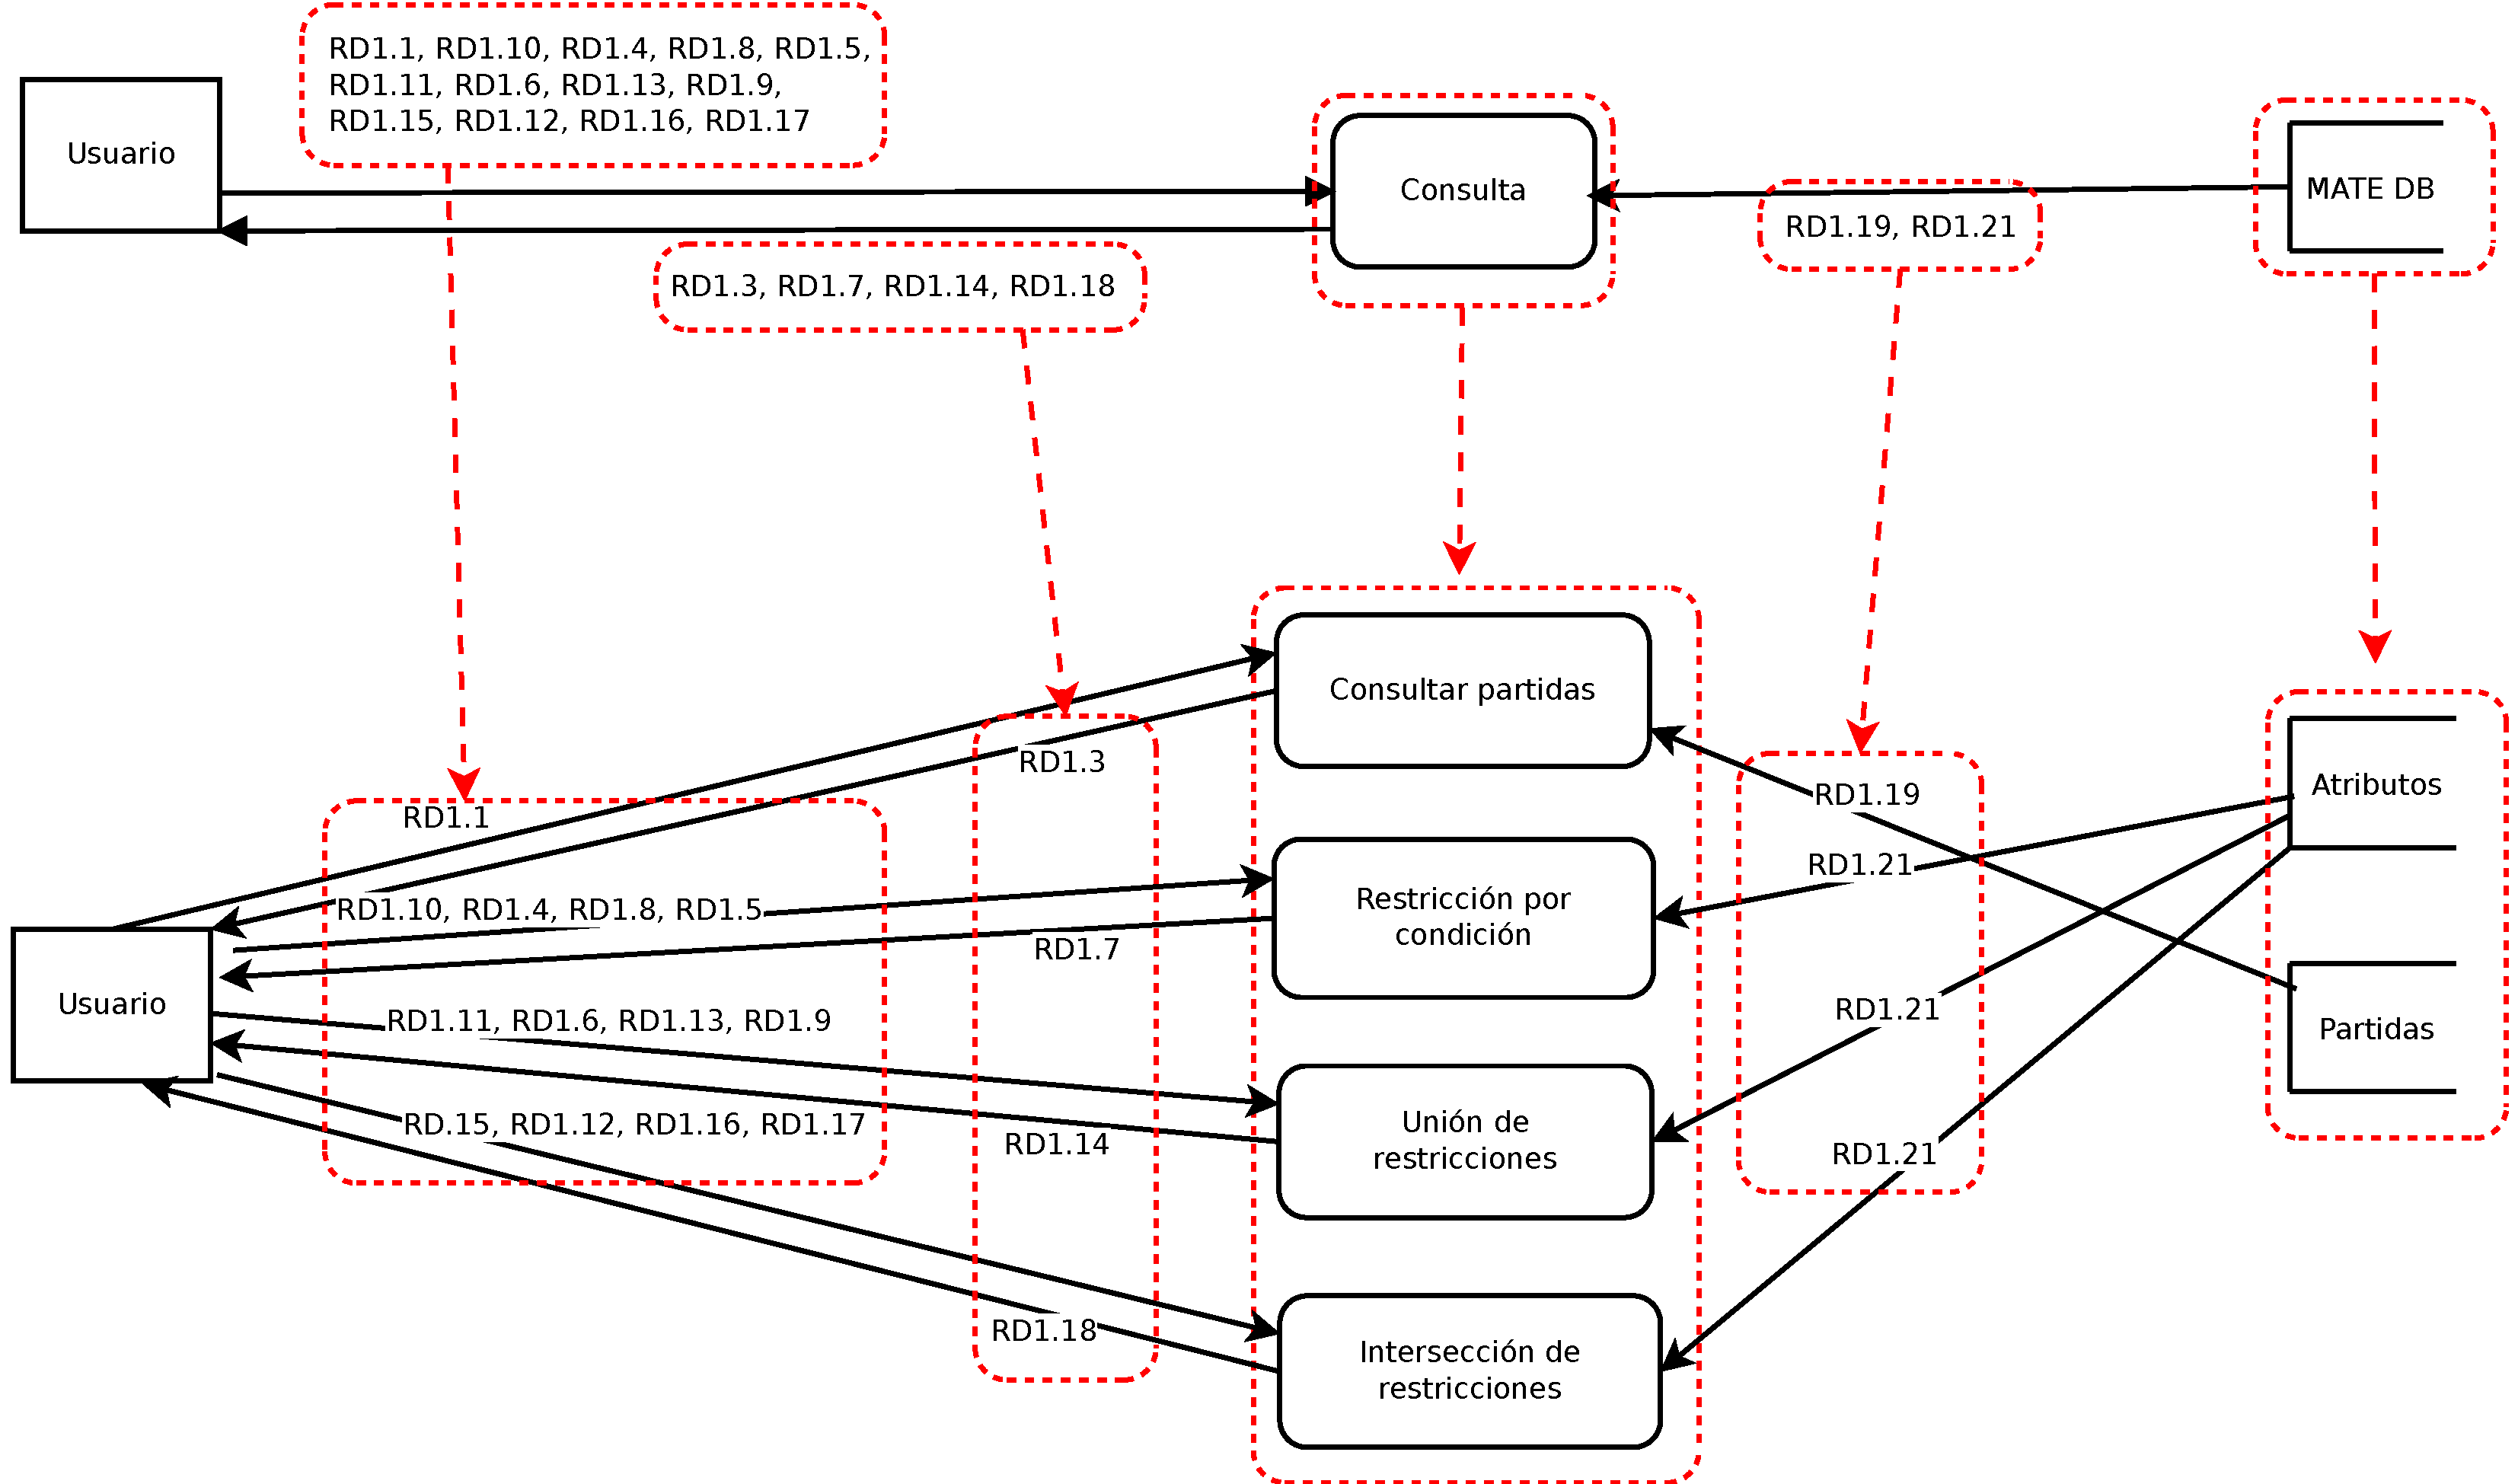
\includegraphics[width=0.7\linewidth]{../Diagramas/pdf/RefinamientoConsulta.pdf}
\caption{Flujo de datos del subsistema Consulta.}

\label{fig:RefinamientoConsulta}
\end{figure}

\subsubsection{Esquema Externo:}

\begin{figure}[h!]
	\centering
	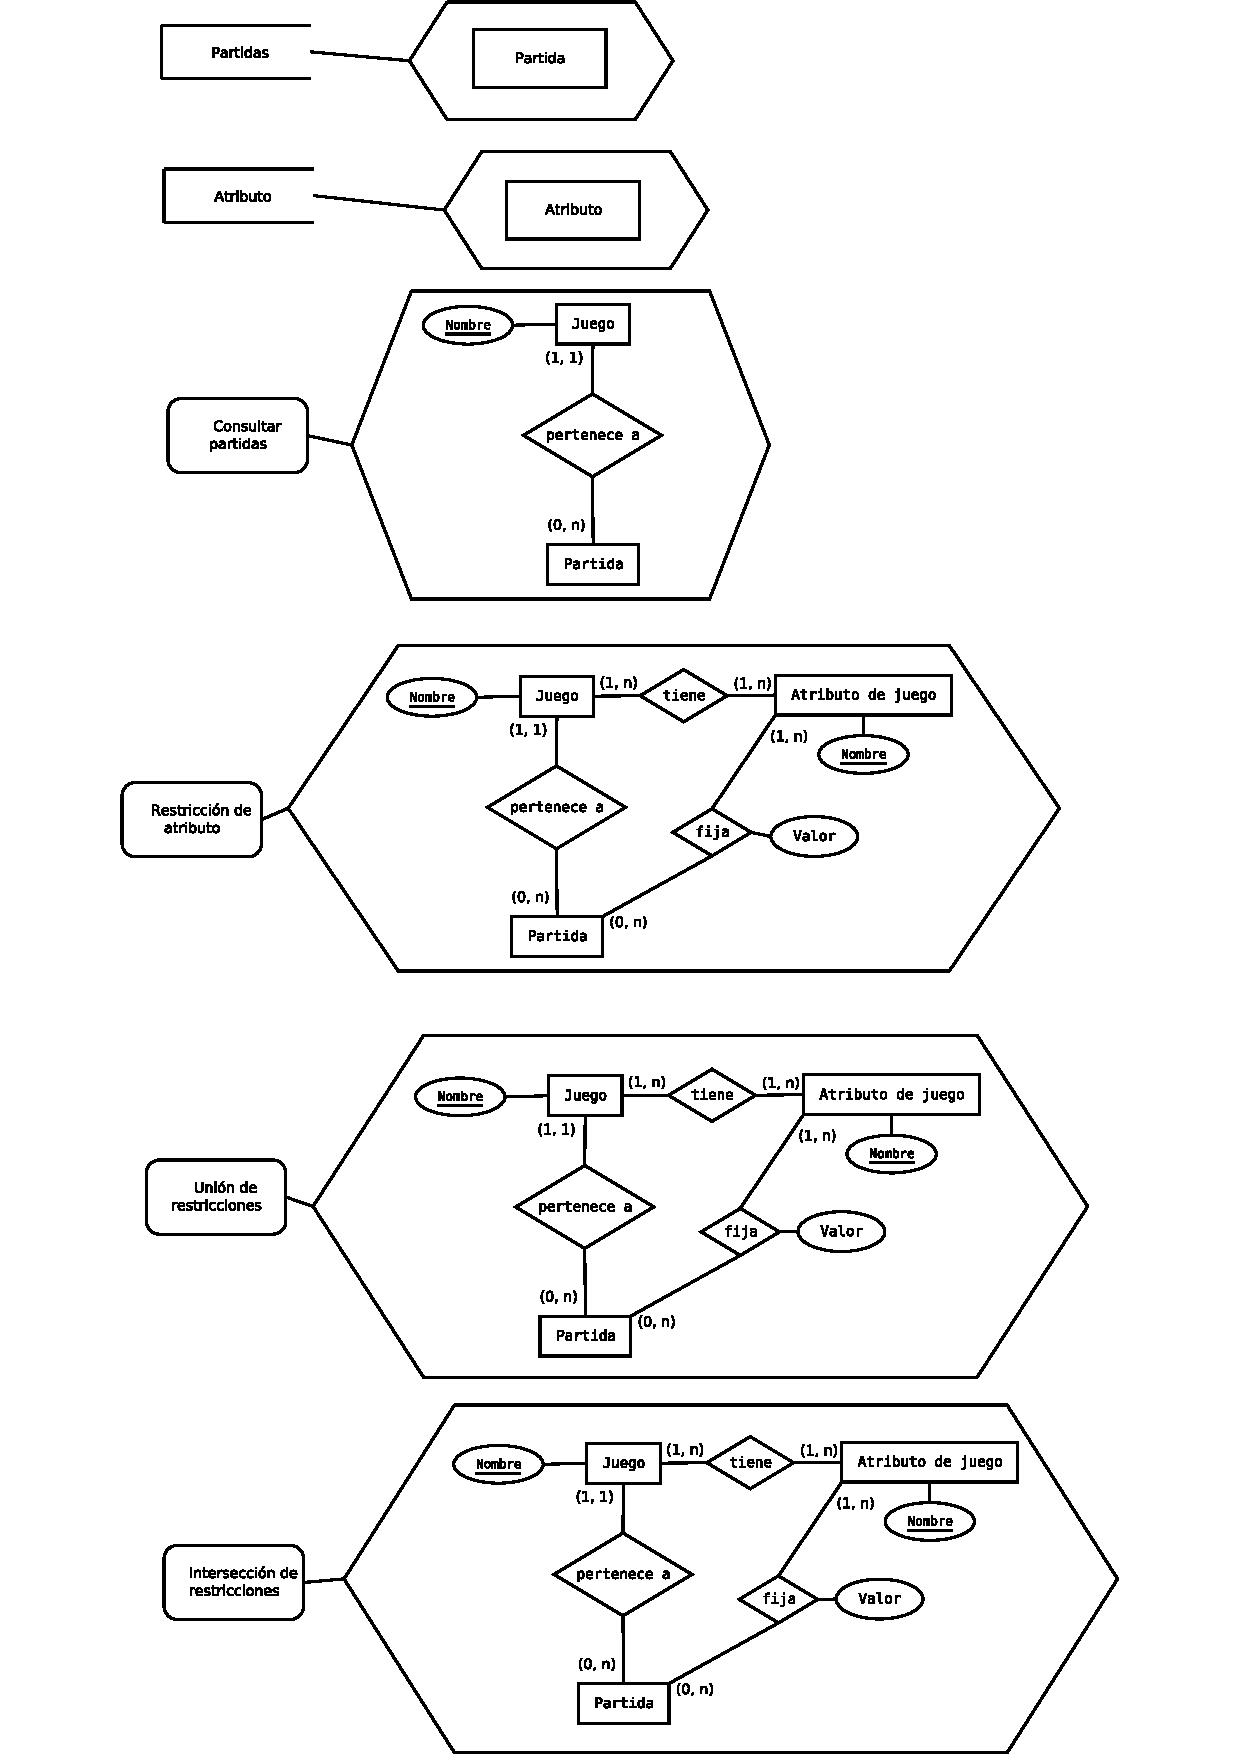
\includegraphics[width=0.7\linewidth]{../Diagramas/pdf/EsquemaExternoConsulta.pdf}
	\caption{Esquema externo de Consulta.}
	
	\label{fig:EsquemaExtConsulta}
\end{figure}


\subsection{Segundo subsistema, consejos}
\subsubsection{Proceso: Recomendar atributos contra un oponente}

\begin{itemize}
	\item \textbf{O1:} Busca las partidas jugadas por un jugador dado el nombre del juego y
		el nombre del jugador.\\

	\item \textbf{O2:} Busca los valores, en las patridas obtenidas
		en O1, de varios atributos dados sus nombres.\\
\end{itemize}

\begin{figure}[h!]
	\centering
	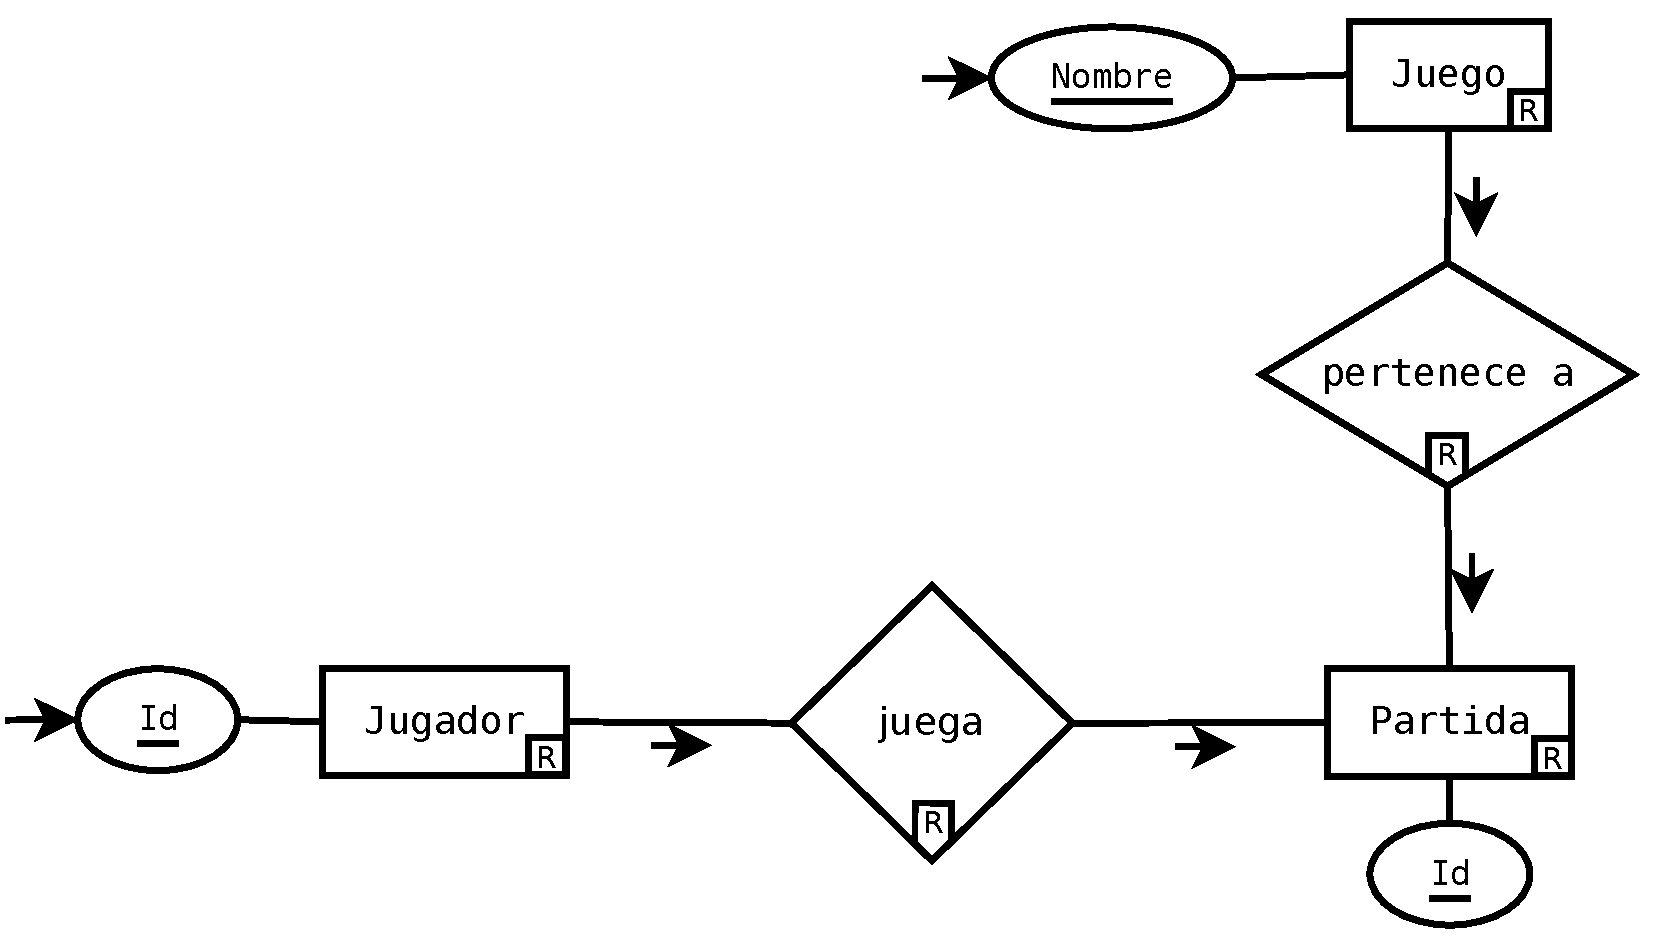
\includegraphics[width=0.5\linewidth]{../Diagramas/pdf/Op1-1.pdf}
	\caption{Esquema de navegabilidad de O1 del proceso 1}
\end{figure}

\begin{figure}[h!]
	\centering
	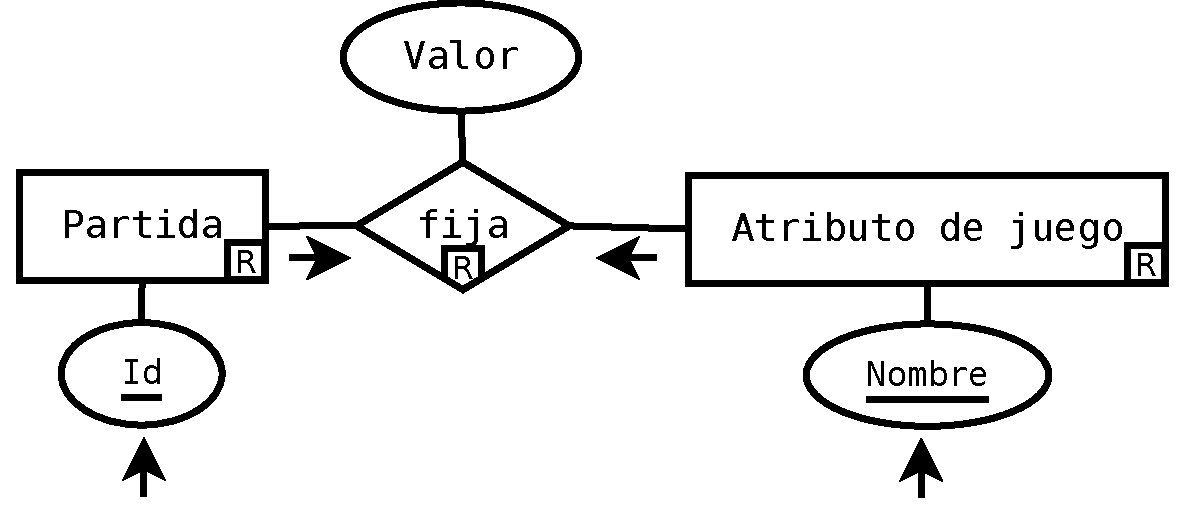
\includegraphics[width=0.5\linewidth]{../Diagramas/pdf/Op1-2.pdf}
	\caption{Esquema de navegabilidad de O2 del proceso 1}
\end{figure}



\subsubsection{Proceso: Recomendar estilo de juego parecido al de un jugador}

\begin{itemize}
	\item \textbf{O1:} Busca las partidas jugadas por un jugador dado el nombre del juego y
		el nombre del jugador.\\
	\item \textbf{O2:} Busca los valores, en las patridas obtenidas
		en O1, de varios atributos dados sus nombres.\\
\end{itemize}

\begin{figure}[h!]
	\centering
	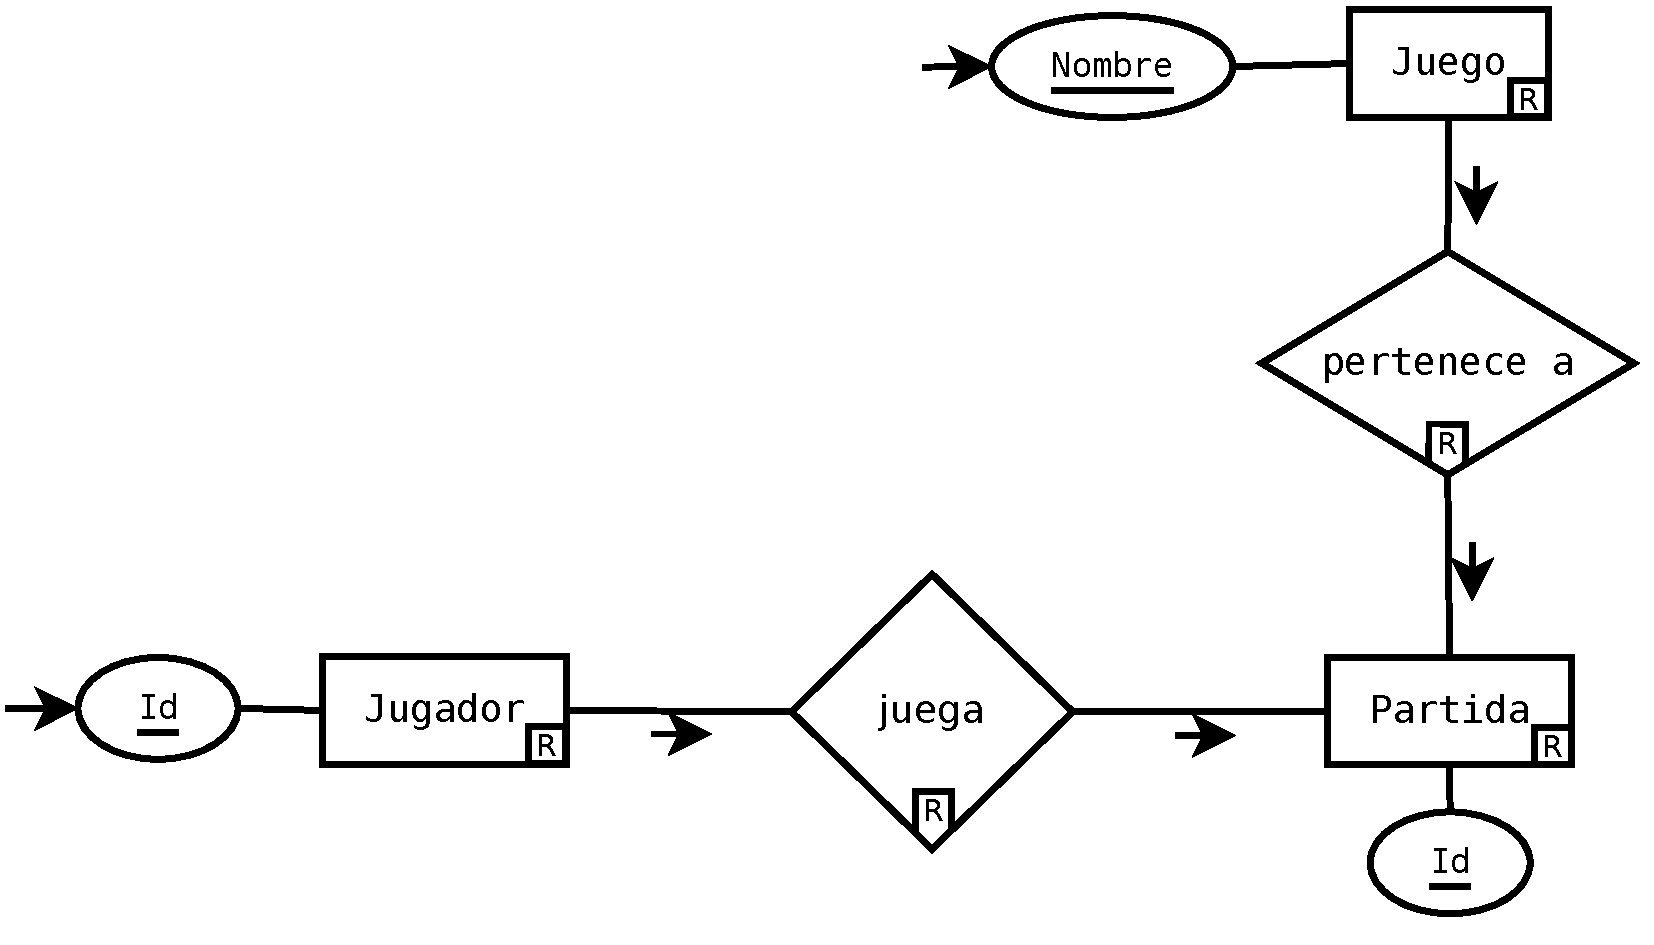
\includegraphics[width=0.5\linewidth]{../Diagramas/pdf/Op2-1.pdf}
	\caption{Esquema de navegabilidad de O1 del proceso 2}
\end{figure}

\begin{figure}[h!]
	\centering
	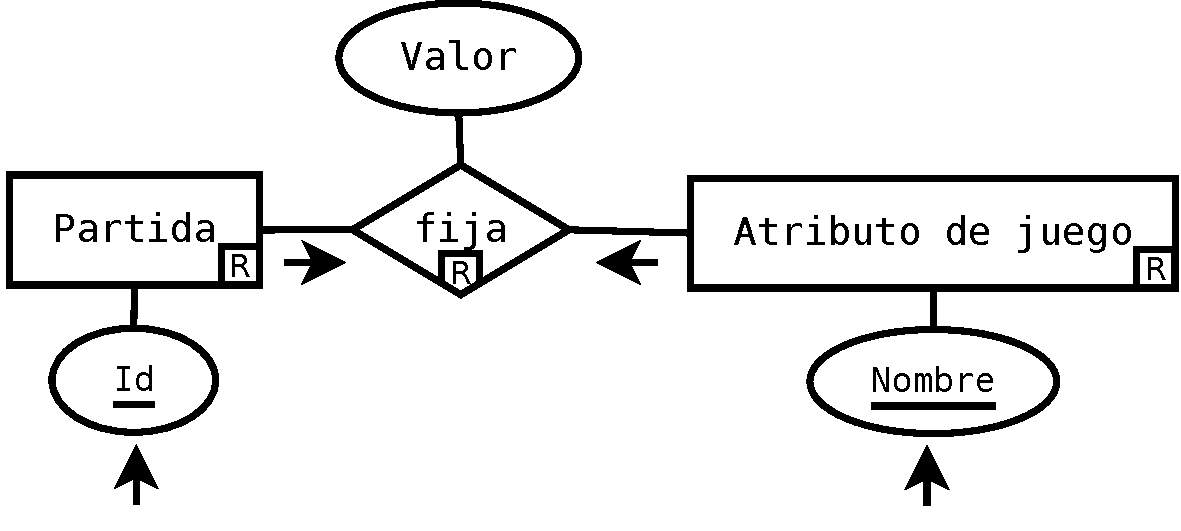
\includegraphics[width=0.5\linewidth]{../Diagramas/pdf/Op2-2.pdf}
	\caption{Esquema de navegabilidad de O2 del proceso 2}
\end{figure}



\subsubsection{Proceso: Recomendar atributos con contexto}

\begin{itemize}
	\item \textbf{O1:} Dado un nombre de juego y el nombre de varios
		atributos junto con un valor asociado a cada uno, 
		buscar las partidas en las que atributo y valor coincidan.\\
	\item \textbf{O2:} Dados varios nombres de atributos, buscar en las
		partidas obtenidas en O1 los valores correspondiantes a
		estos.\\
\end{itemize}

\begin{figure}[h!]
	\centering
	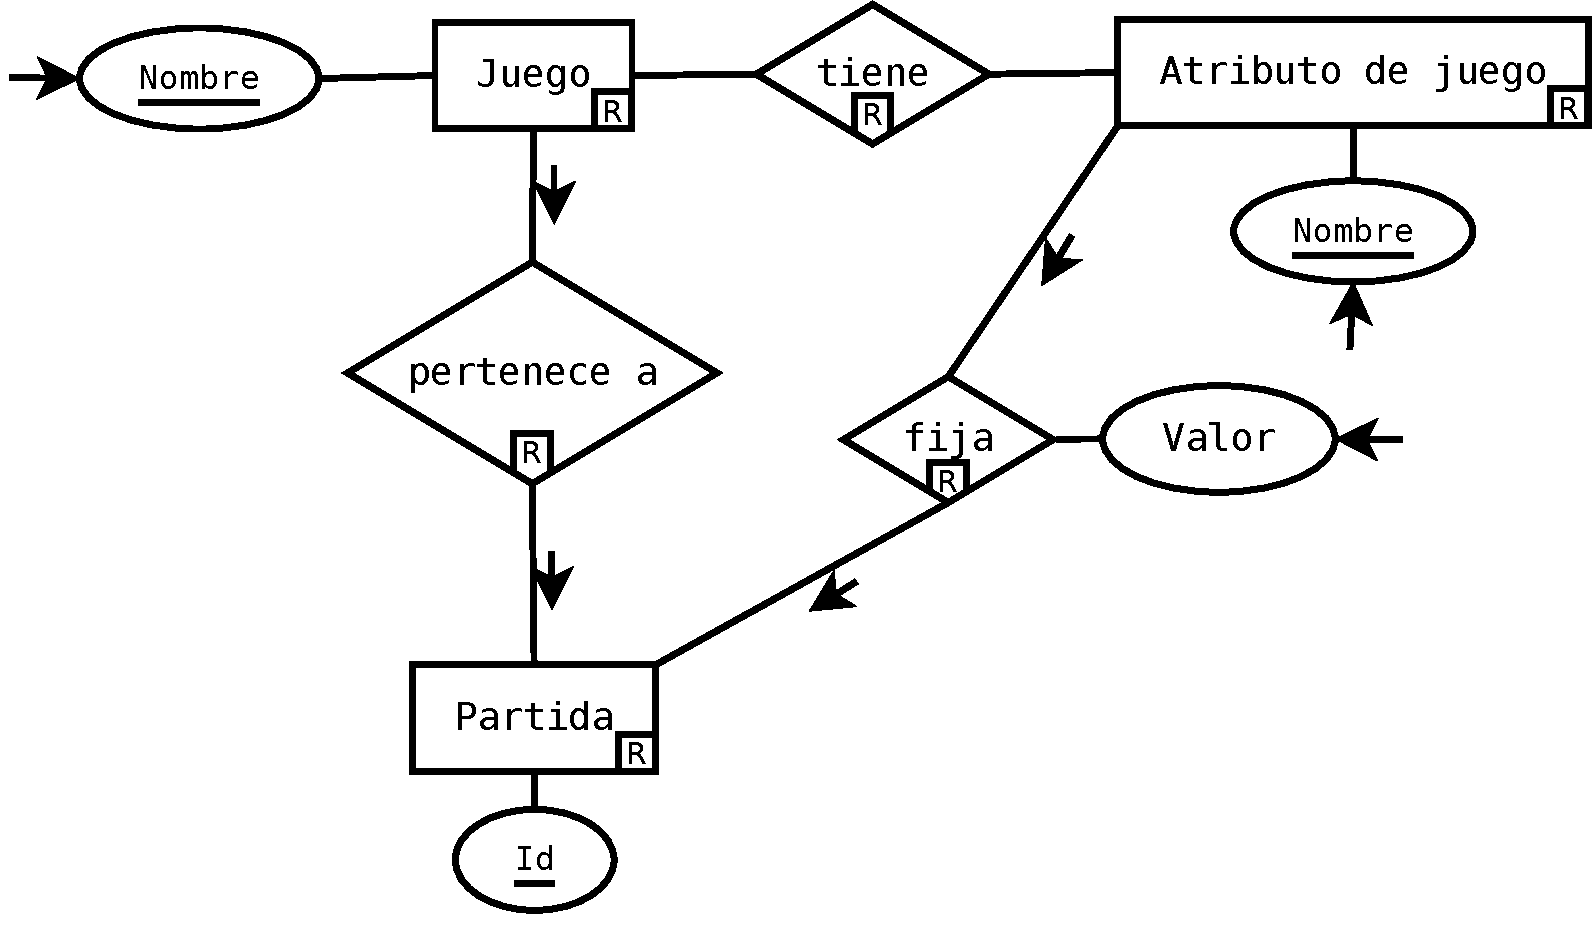
\includegraphics[width=0.5\linewidth]{../Diagramas/pdf/Op3-1.pdf}
	\caption{Esquema de navegabilidad de O1 del proceso 3}
\end{figure}

\begin{figure}[h!]
	\centering
	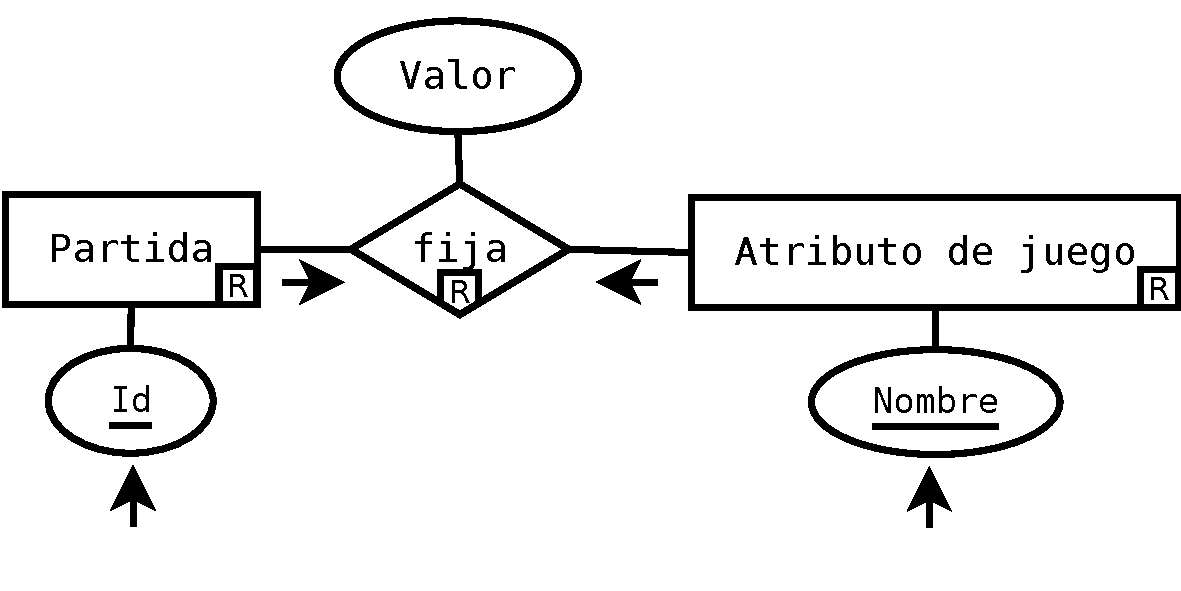
\includegraphics[width=0.5\linewidth]{../Diagramas/pdf/Op3-2.pdf}
	\caption{Esquema de navegabilidad de O2 del proceso 3}
\end{figure}



\subsubsection{Proceso: Recomendar atributos en general}

\begin{itemize}
	\item \textbf{O1:} Dado el nombre de un juego, el nombre de varios atributos y una puntuación
		, buscar los valores de los atributos anteriores en todas las partidas del juego
		que los contengan y cuya puntuación sea mayor que la dada, junto con la puntuación
		de esa partida.\\
\end{itemize}

\begin{figure}[h!]
	\centering
	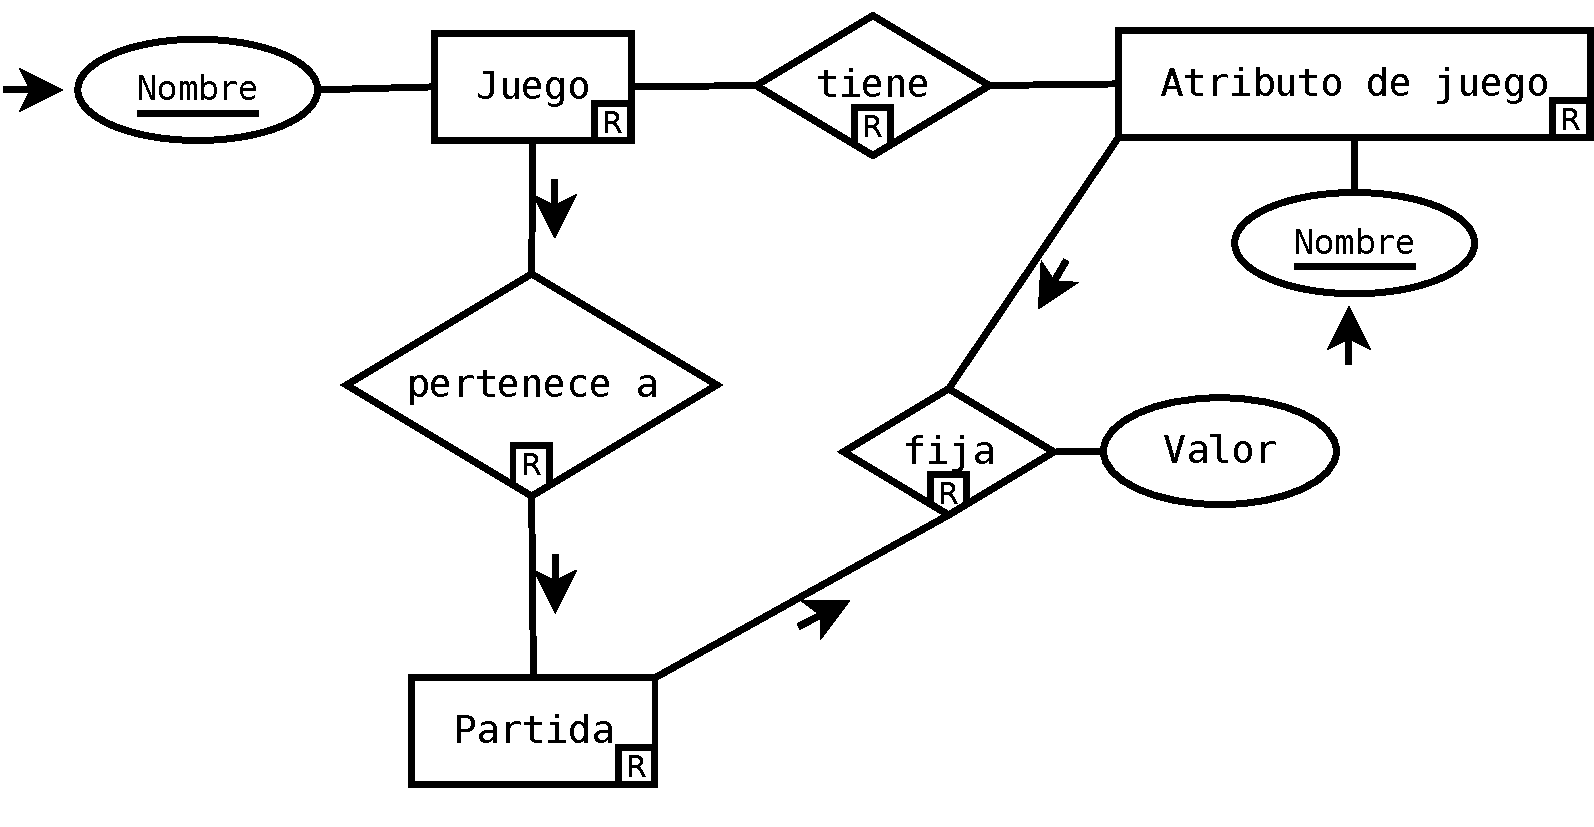
\includegraphics[width=0.5\linewidth]{../Diagramas/pdf/Op4-1.pdf}
	\caption{Esquema de navegabilidad de O1 del proceso 4}
\end{figure}



\subsection{ Tercer subsistema, inclusión}
\subsection{Esquemas de navegabilidad del sistema de inclusión}
\begin{itemize}
  \item \textbf{Inclusion de partidas}
  \begin{figure}[H]
    \centering
    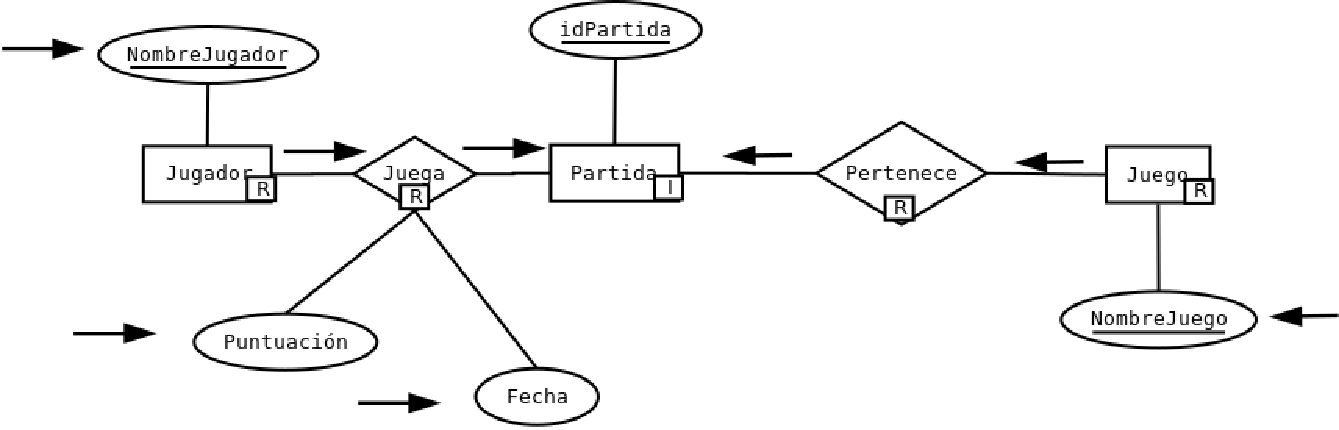
\includegraphics[width=0.5\linewidth]{../Diagramas/pdf/IncluirPartida.pdf}
    \caption{Esquema de navegabilidad de del proceso 1}
  \end{figure}

  \item \textbf{Modificación de partidas}
  \begin{figure}[H]
    \centering
    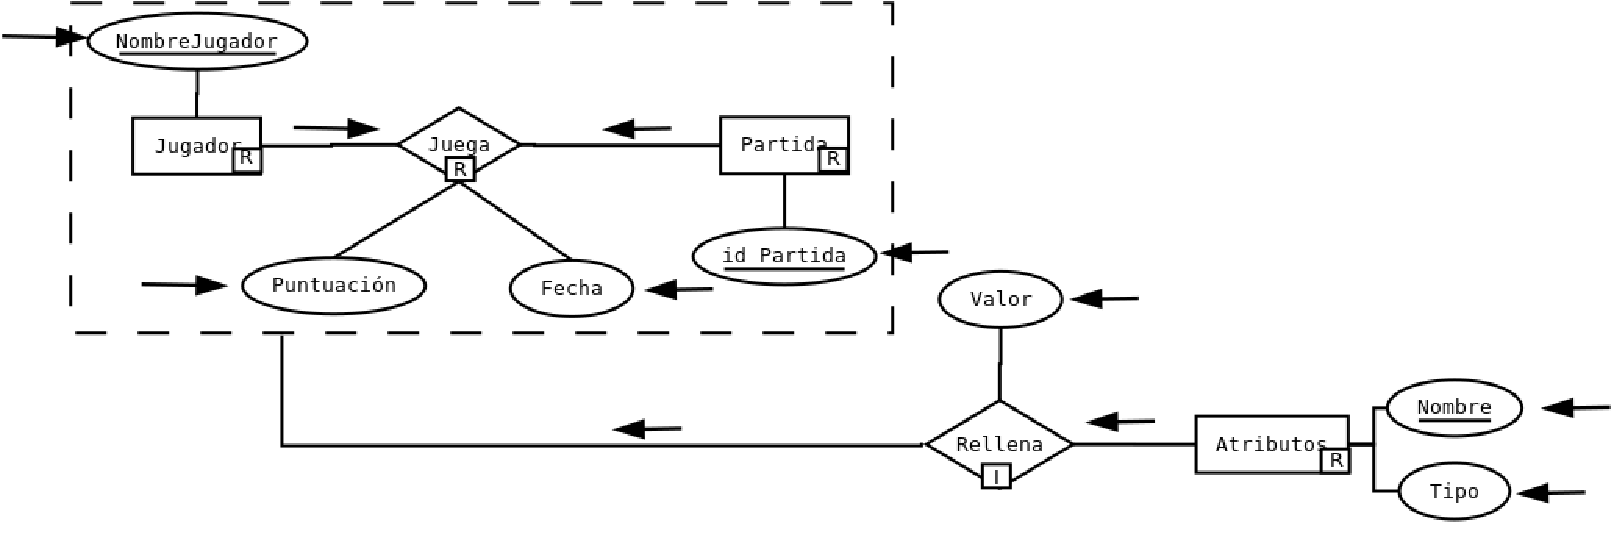
\includegraphics[width=0.5\linewidth]{../Diagramas/pdf/ModificarPartida.pdf}
    \caption{Esquema de navegabilidad del proceso 2}
  \end{figure}

  \item \textbf{Eliminación de partidas}
  \begin{figure}[H]
    \centering
    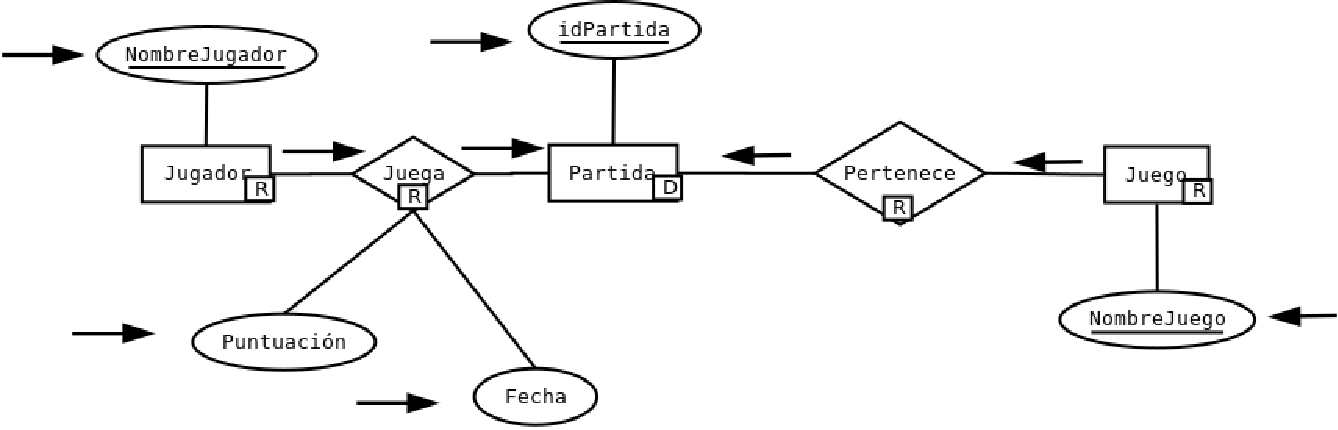
\includegraphics[width=0.5\linewidth]{../Diagramas/pdf/EliminarRegistro.pdf}
    \caption{Esquema de navegabilidad del proceso 2}
  \end{figure}

  \item \textbf{Comentar la partida de otro jugador}
  \begin{figure}[H]
    \centering
    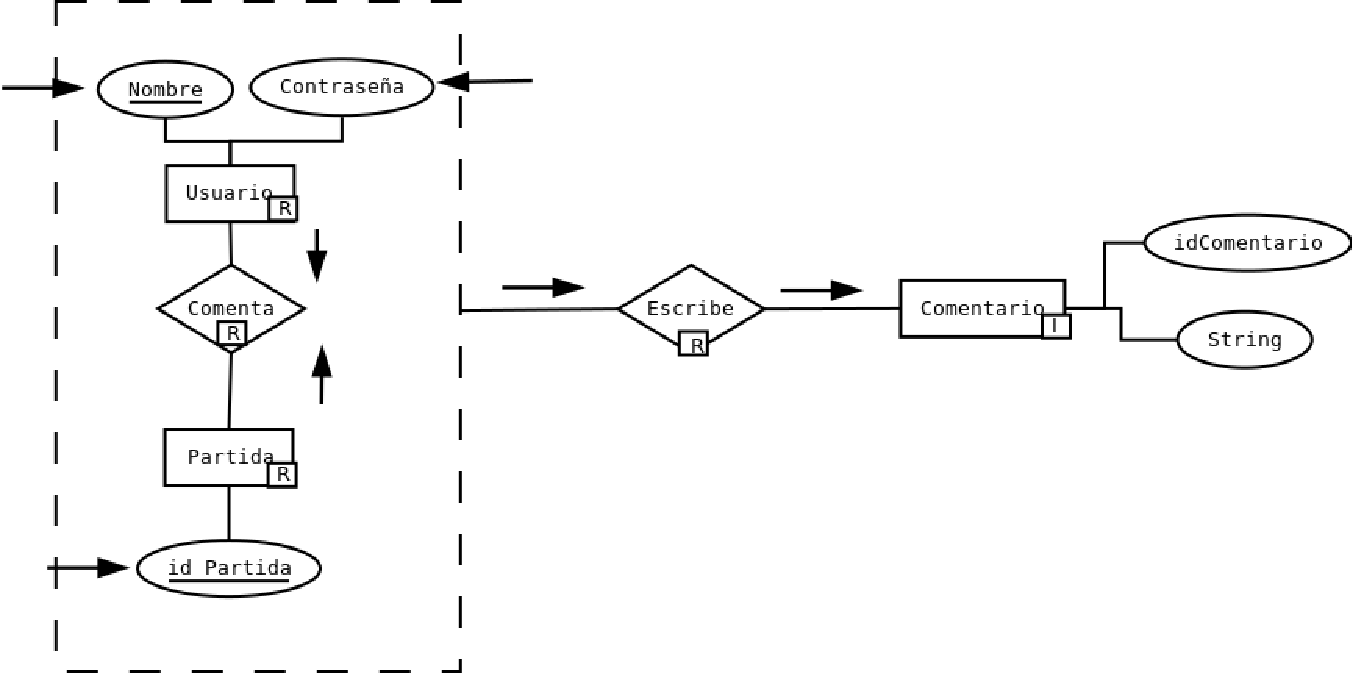
\includegraphics[width=0.5\linewidth]{../Diagramas/pdf/ComentarPartida.pdf}
    \caption{Esquema de navegabilidad del proceso 2}
  \end{figure}


\end{itemize}


\subsection{Cuarto subsistema, estadísticas}
\subsubsection{Proceso: Realizar gráfica 2D}

\begin{itemize}
	\item \textbf{O1:} Busca los valores de los atributos a partir del nombre y del nombre del juego, y consigue la tupla fecha, valor, nombre de jugador.
\end{itemize}

\begin{figure}[H]
	\centering
	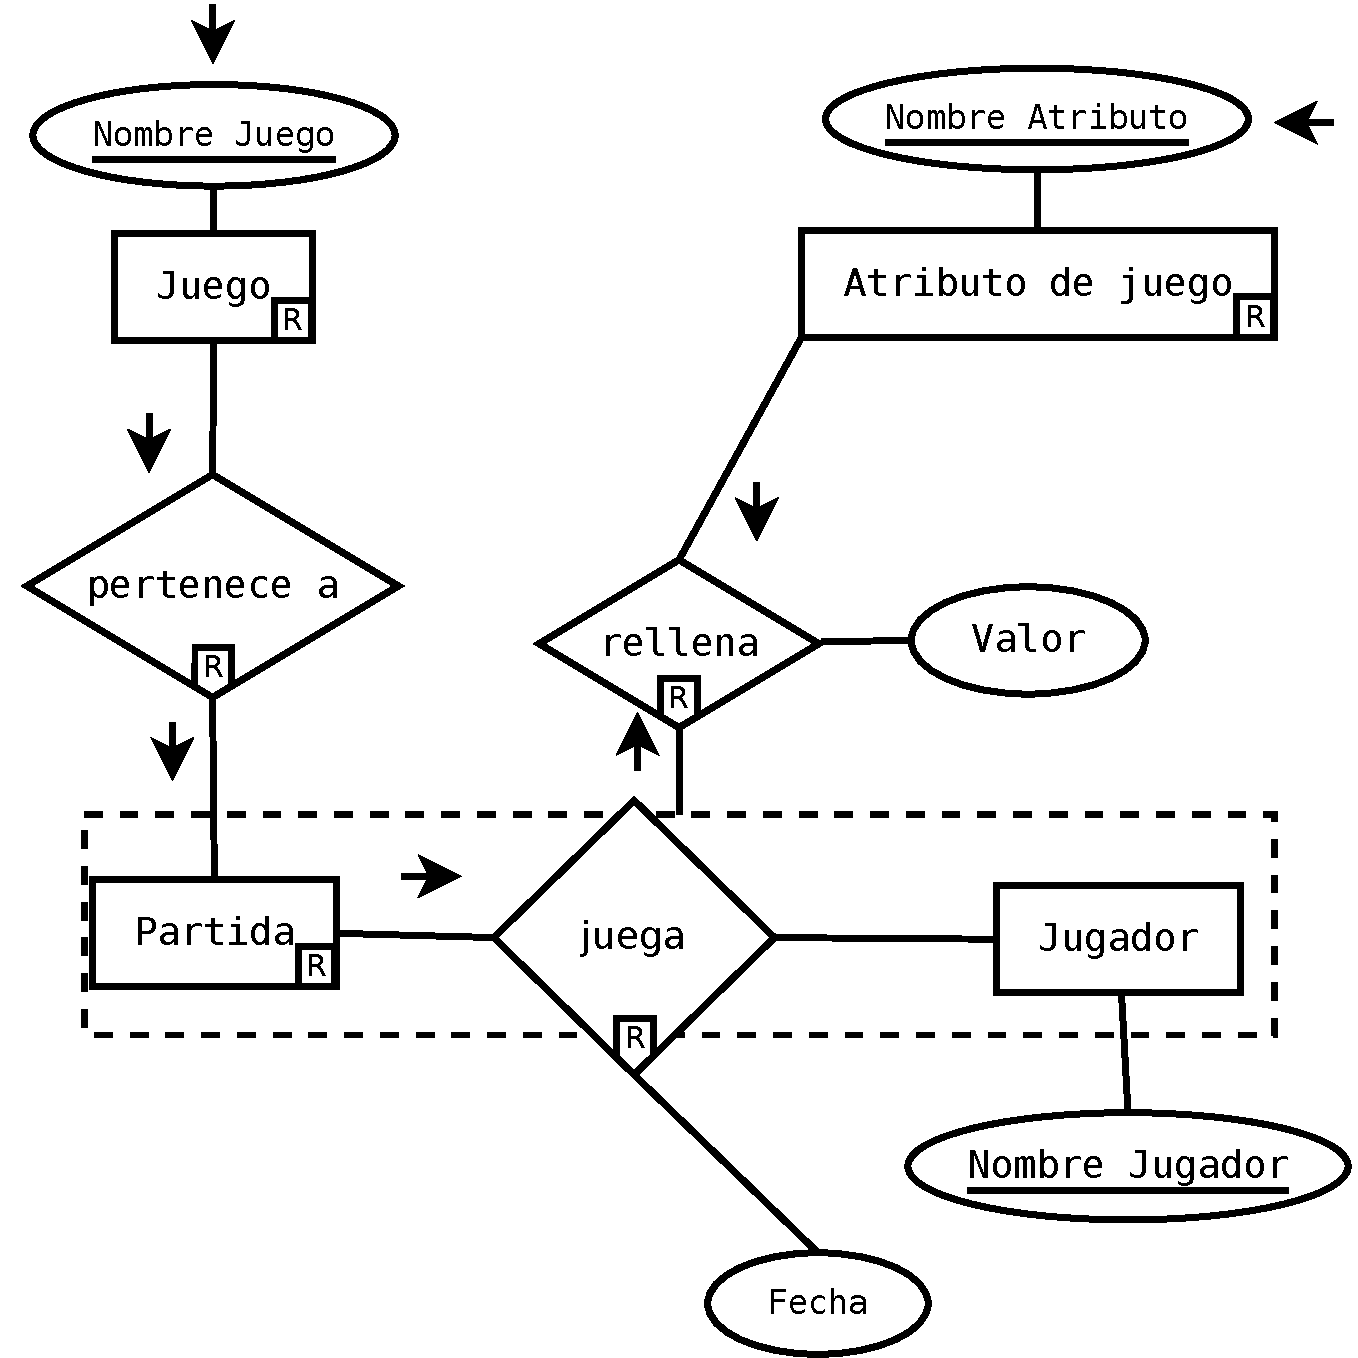
\includegraphics[width=0.5\linewidth]{../Diagramas/pdf/OpEstadisticas3.pdf}
	\caption{Esquema de navegabilidad  O1 del proceso 4.1}
	
	\label{fig:O4.1}
\end{figure}
 \begin{itemize}
 	\item \textbf{O2:} Con los valores anteriores, se ha realizado una gráfica que con esta operación insertamos. Conseguimos el usuario que está haciendo la estadística, la imagen de ella y su id, y la insertamos de forma correcta en la base de datos.
 \end{itemize}

\begin{figure}[H]
	\centering
	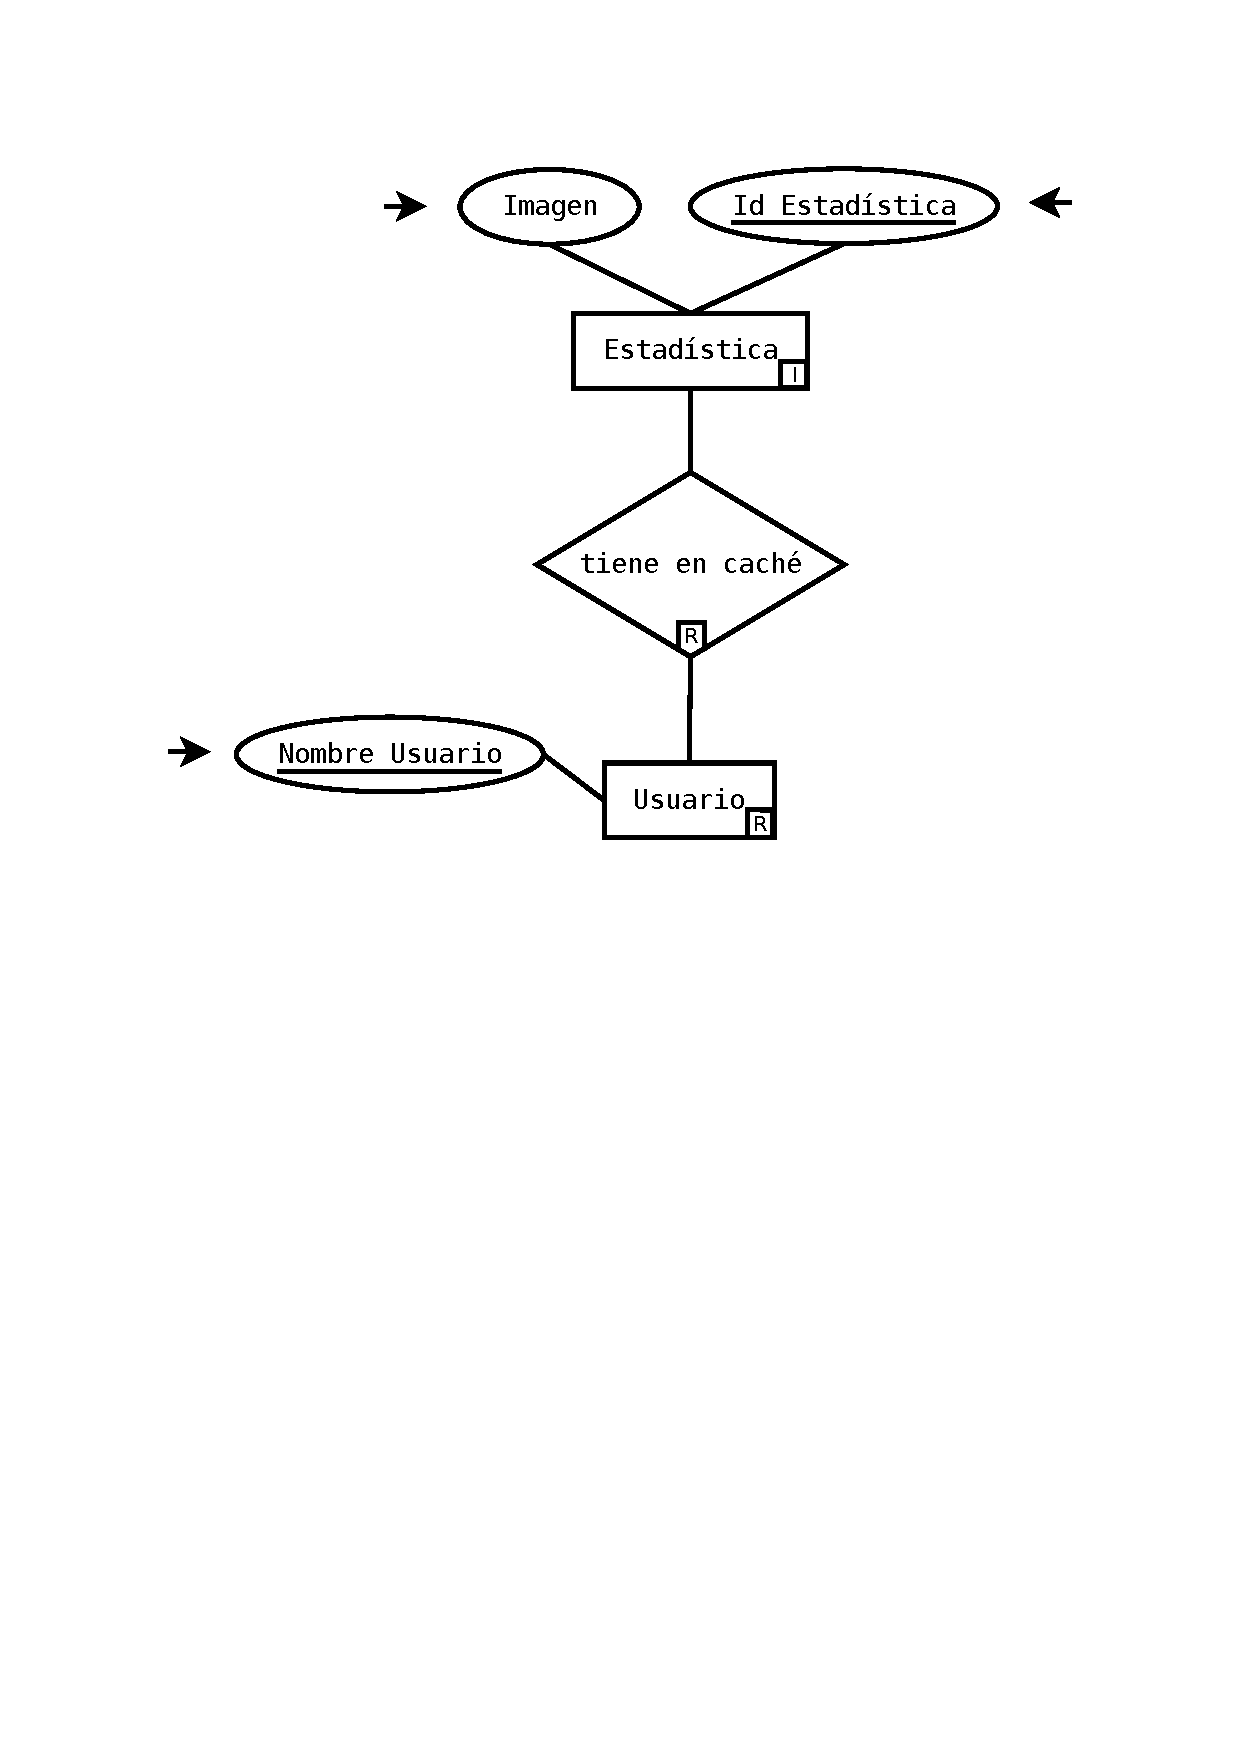
\includegraphics[width=0.5\linewidth]{../Diagramas/pdf/OpEstadisticas1-2.pdf}
	\caption{Esquema de navegabilidad  O2 del proceso 4.1}
	
	\label{fig:O4.12}
\end{figure}





\newpage
\subsection{Dependencias Funcionales}
\begin{itemize}
	\subsubsection{Iñaki}
\item{{\large Tiene\_en\_Caché}}\\
	$R = \{idEstadistica,nombreUsuario\}$\\
	$DF_1 = \{idEstadistica \rightarrow nombreUsuario\}$\\

\item {{\large Usuario}}\\
	$R = \{nombre, password\}$\\
	$DF_1 = \{nombre \rightarrow password\}$\\

\item{{\large Tiene}}\\
	$R = \{nombreJuego, nombreAtributo\}$\\
	$DF_1 = \{\}$

\subsubsection{Bruno}
\item{{\large Partida}}\\
	$R = \{id\}$\\
	$DF_1 = \{\}$\\

\item {{\large Resume}}\\
	$R = \{idEstadistica, nombreJuego\}$\\
	$DF_1 = \{idEstadistica \rightarrow nombreJuego\}$\\

\item{{\large Rellena}}\\
	$R = \{idPartida, nombreJugador, nombreAtributo, valor\}$\\
	$DF_1 = \{\{idPartida, nombreJugador, nombreAtributo\} \rightarrow valor\}$

\subsubsection{Darío}
\item{\large{Juego}} \\
$R = \{nombre \} $ \\
$DF_1 = \{\}$\\

\item{\large{Juega}} \\
$R = \{nombreJugador, idPartida, puntuacion,fecha \} $ \\
$DF_1 = \{ \{nombreJugador,idPartida \} \rightarrow puntuacion,fecha\}$ \\

Está en FNBC porque $(idEstadistica,idPartida)$ es clave candidata y $puntuacion$y $fecha$ no están contenidas en ella.

\item{\large{Pertenece}}\\
$R = \{idPartida,nombreJuego\} $\\
$DF_1 = \{ \{idPartida\} \rightarrow nombreJuego \}$\\
Está en FNBC porque $idPartida$ es clave candidata y $nombreJuego$ no está contenido en ella.

\item{\large{Jugador}}\\
$R = \{nombre\} \\
$ DF_1 = \{\} $ \\

Todas las tablas están normalizadas ya que presentan una única dependencia funcional.

\subsubsection{Antonio}
\item{{\large Estadistica}}\\
$R = \{id, imagen\}$\\
$DF_1 = \{id \rightarrow imagen\}$\\
Esta tabla ya está en FNBC, id es una clave candidata (en este caso la única), e imagen no está contenida en ella. Además, al haber una sola dependencia funcional no hay transitivas problemáticas y todos los elementos no primos, en este caso imagen, dependen completamente de la clave candidata, ya que solo hay un elemento en ella.

\item {{\large Atributo}}\\
$R = \{nombre, tipo\}$\\
$DF_1 = \{nombre \rightarrow tipo\}$\\
Esta tabla ya está en FNBC, nombre es una clave candidata (en este caso la única), y tipo no está contenido en él. Además, al haber una sola dependencia funcional no hay transitivas problemáticas y todos los elementos no primos, en este caso tipo, dependen completamente de la clave candidata, ya que solo hay un elemento en ella.

\item{{\large Comenta}}\\
$R = \{nombreUsuario, idPartida, comentario\}$\\
$DF_1 = \{\}$
Esta tabla ya está en FNBC al no haber dependencias funcionales más que las triviales. Necesitas todo el conjunto para determinar la tupla de comenta. Así que todo el conjunto tiene que ser la clave primaria (y única clave candidata).
\end{itemize}

\end{document}
